%%%%%%%%%%%%%%%%%%%%%
% Experiments and Results %
%%%%%%%%%%%%%%%%%%%%%

This thesis aims to analyze the relationships between different road networks and road network similarity methods. In particular,  (1) the similarities between different road networks are determined, (2) similar road networks are clustered, (3) the correlations between the different network similarity methods used to identify the similarities between the different road networks are also determined, and (4) the similar methods are clustered. Figures \ref{fig:Road Network Similarity and Ranking} and \ref{fig:Road Network Similarity Method Correlation} show a high-level overview of the process. 

\begin{figure}[h]
\centering
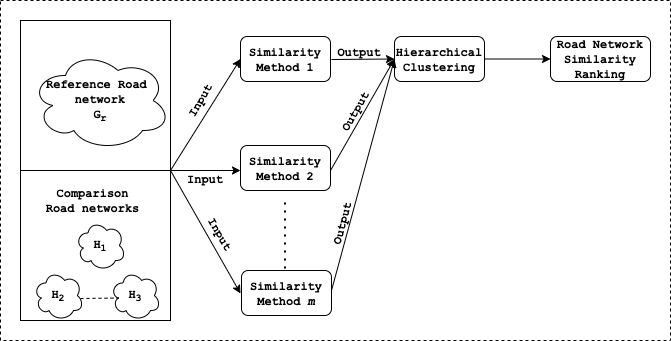
\includegraphics[width=0.75\textwidth,center]{picture/network_ranking.png}
\caption[Road Network Similarity and Ranking]{Road Network Similarity and Ranking}
\label{fig:Road Network Similarity and Ranking}
\end{figure}

\begin{figure}[!ht]
\centering
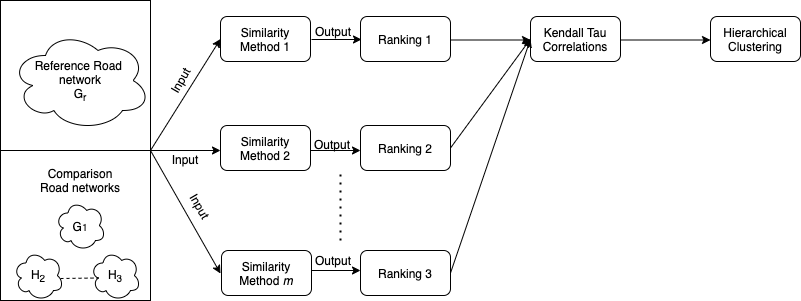
\includegraphics[width=0.75\textwidth,center]{picture/ranking.png}
\caption[Road Network Similarity Method Correlation]{Road Network Similarity Method Correlation}
\label{fig:Road Network Similarity Method Correlation}
\end{figure}


\section{Grid Road Network Similarity Analysis}
\label{4.1}
This section describes the experiments conducted to identify similar road networks with Grid patterns and structure, as well as groups of methods described in Chapter 3 that exhibit similar behavior. It is important to note that the road networks were chosen empirically.

Using network-similarity ranking [\cite{Soundarajan:2014}], the problem of finding road networks with similar structures and patterns is explicitly addressed. First, a reference network $G_r$ and a set of comparison networks $H_1, H_2,...., H_k$ are provided. The similarity between $G_r$ and each $H_i$ is then calculated using a network-similarity method. Before creating a dendrogram, the data (similarity scores) for each comparison are normalized for uniformity. This will cancel out the effects of outliers and ensure that the results are all in the same unit. The similarity score for each comparison is shown in figure \ref{fig:Heatmap showing the correlations for Grid Road Networks}, and the normalization is accomplished by calculating Z scores for each similarity score in each column: $z = (x mean)/std$. As a result, the column mean is subtracted from each column value and divided by the standard deviation. As a result, the mean and variance for all columns are the same. The normalized values show how many standard deviations each individual value is from the column mean. By combining the linkage function to generate the dendrogram, the hierarchical clustering algorithm can now be used in conjunction with the Ward Variance Minimization algorithm.

For the Grid road similarity analysis, the District of Columbia (USA) is chosen as the reference network, and the methods are used to compare the other networks to the reference network and generate a numerical similarity score. The networks are then organized into hierarchical clusters. The goal is to see if specific road networks have Grid patterns that are similar to the reference network's Grid pattern, which results in a dendrogram with road network patterns that are similar to the reference road network pattern. Figure \ref{fig:Hierarchical Clustering Dendrogram for Grid Road Networking Similarity} shows the results of this analysis.

\begin{figure}[!ht]
\centering
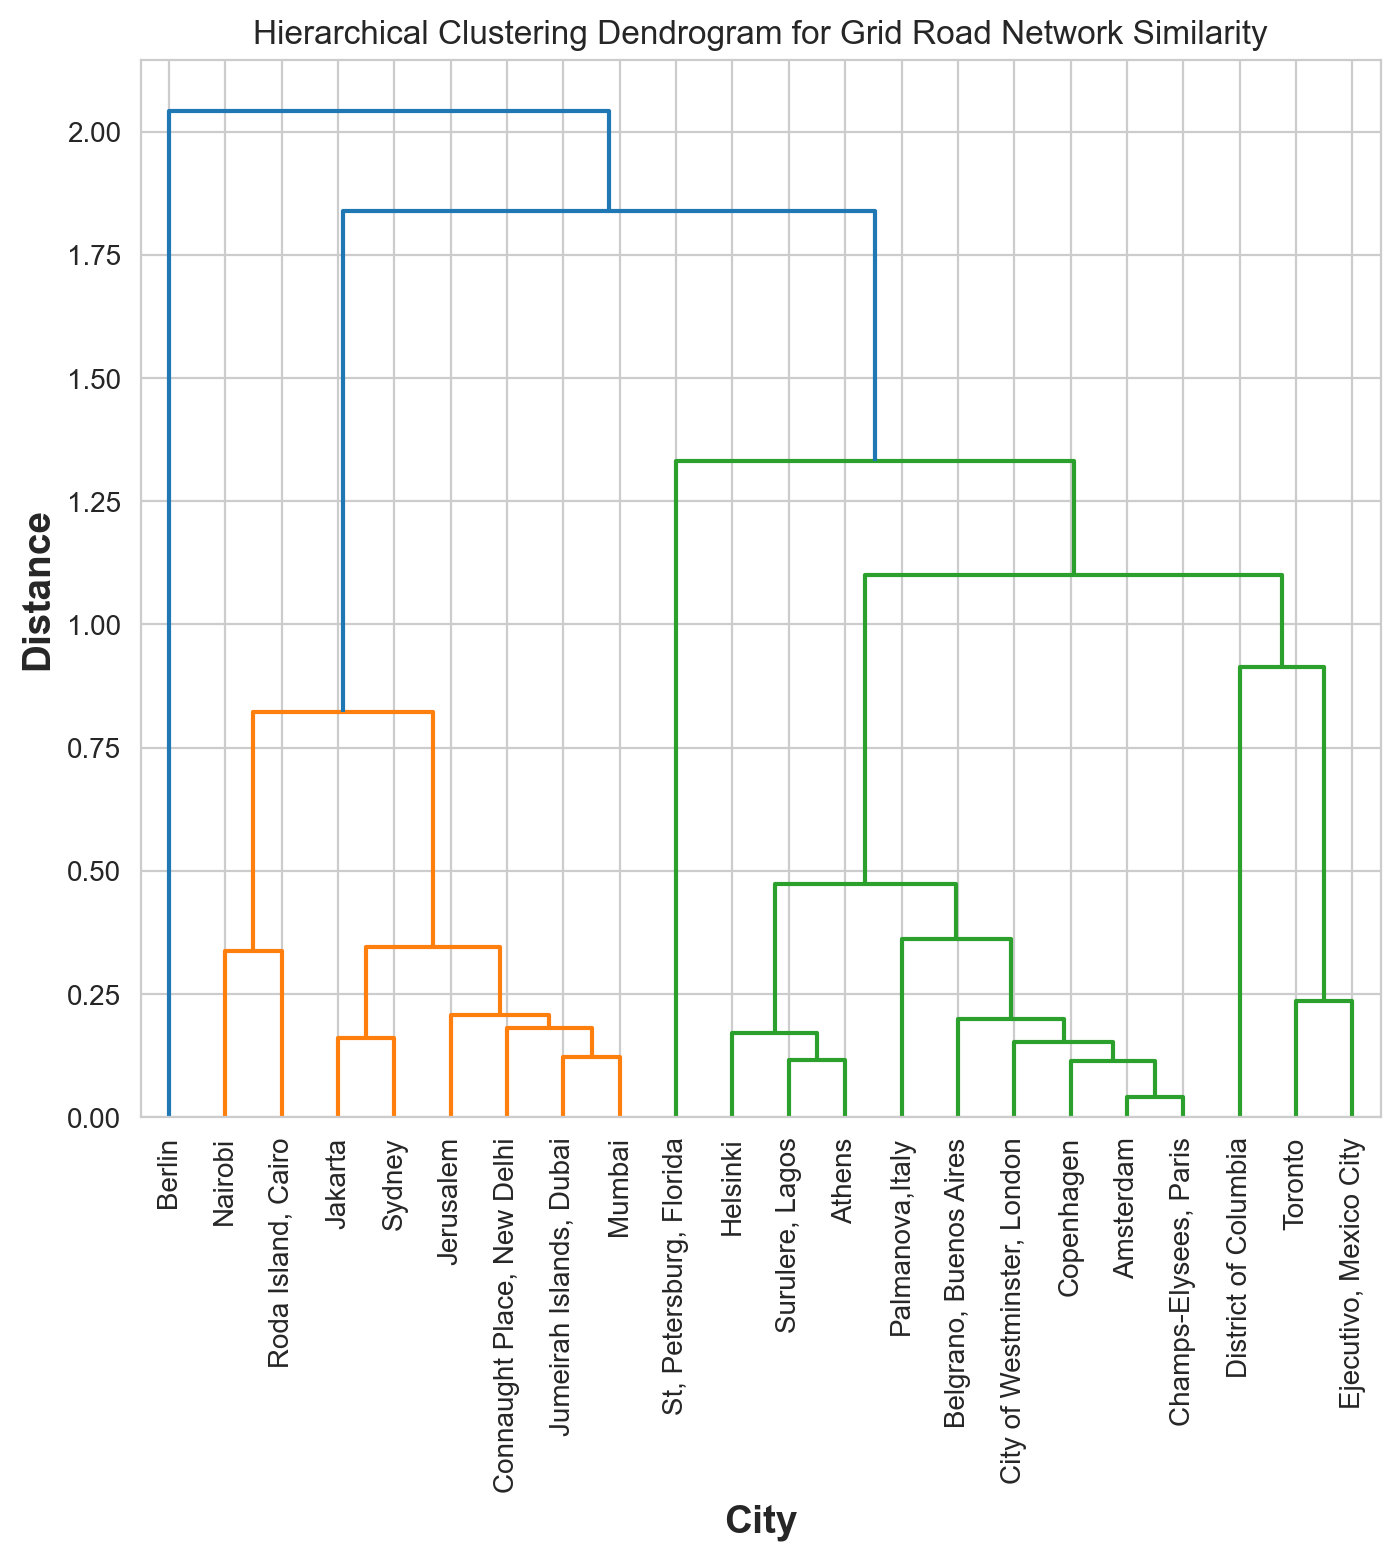
\includegraphics[width=0.75\textwidth,center]{picture/Grid/grid_dendrogram2.png}
\caption[Hierarchical Clustering Dendrogram for Grid Road Networking Similarity]{Hierarchical Clustering Dendrogram for Grid Road Networking Similarity}
\label{fig:Hierarchical Clustering Dendrogram for Grid Road Networking Similarity}
\end{figure}

The dendrogram obtained from the cluster analysis is shown in figure \ref{fig:Hierarchical Clustering Dendrogram for Grid Road Networking Similarity}. Two criteria are used to interpret the dendrogram. First, a branch or cluster of comparative networks that also contains the reference network. Second, the cluster arrangement that tells us which road networks are the most similar to each other, as the height of the cluster measured in distance indicates how similar or different the road networks are. The larger the difference, the greater the distance.

For the first criteria, two major clusters (Green and Orange) can be observed from the dendrogram's structure except for the outlier; berlin road network (Blue). Looking at the green cluster, the road networks for Ejecutivo and Toronto are adjacent to the reference network: District of Columbia (USA) in one cluster and are later grouped as a single cluster, indicating that these cities have the most pronounced grid-like structure similar to the reference network. 
Using the second criteria to interpret the dendrogram, the road networks of the cities Champs-Elysees, Paris, and Amsterdam, Netherlands are said to be clustered first because they have the cluster with the shortest distance. As a result, they are more similar than any other cluster of road networks in the dendrogram.

At first glance, the road networks within the green cluster should have similarities the grid pattern of the reference network and have clusters with the shortest distance, but by comparing the similarity scores for each method included in the heatmap in figure \ref{fig:Heatmap showing the correlations for Grid Road Networks}, it is possible to determine the characteristics of each cluster and why certain clusters are grouped together.

\begin{figure}[!ht]
\centering
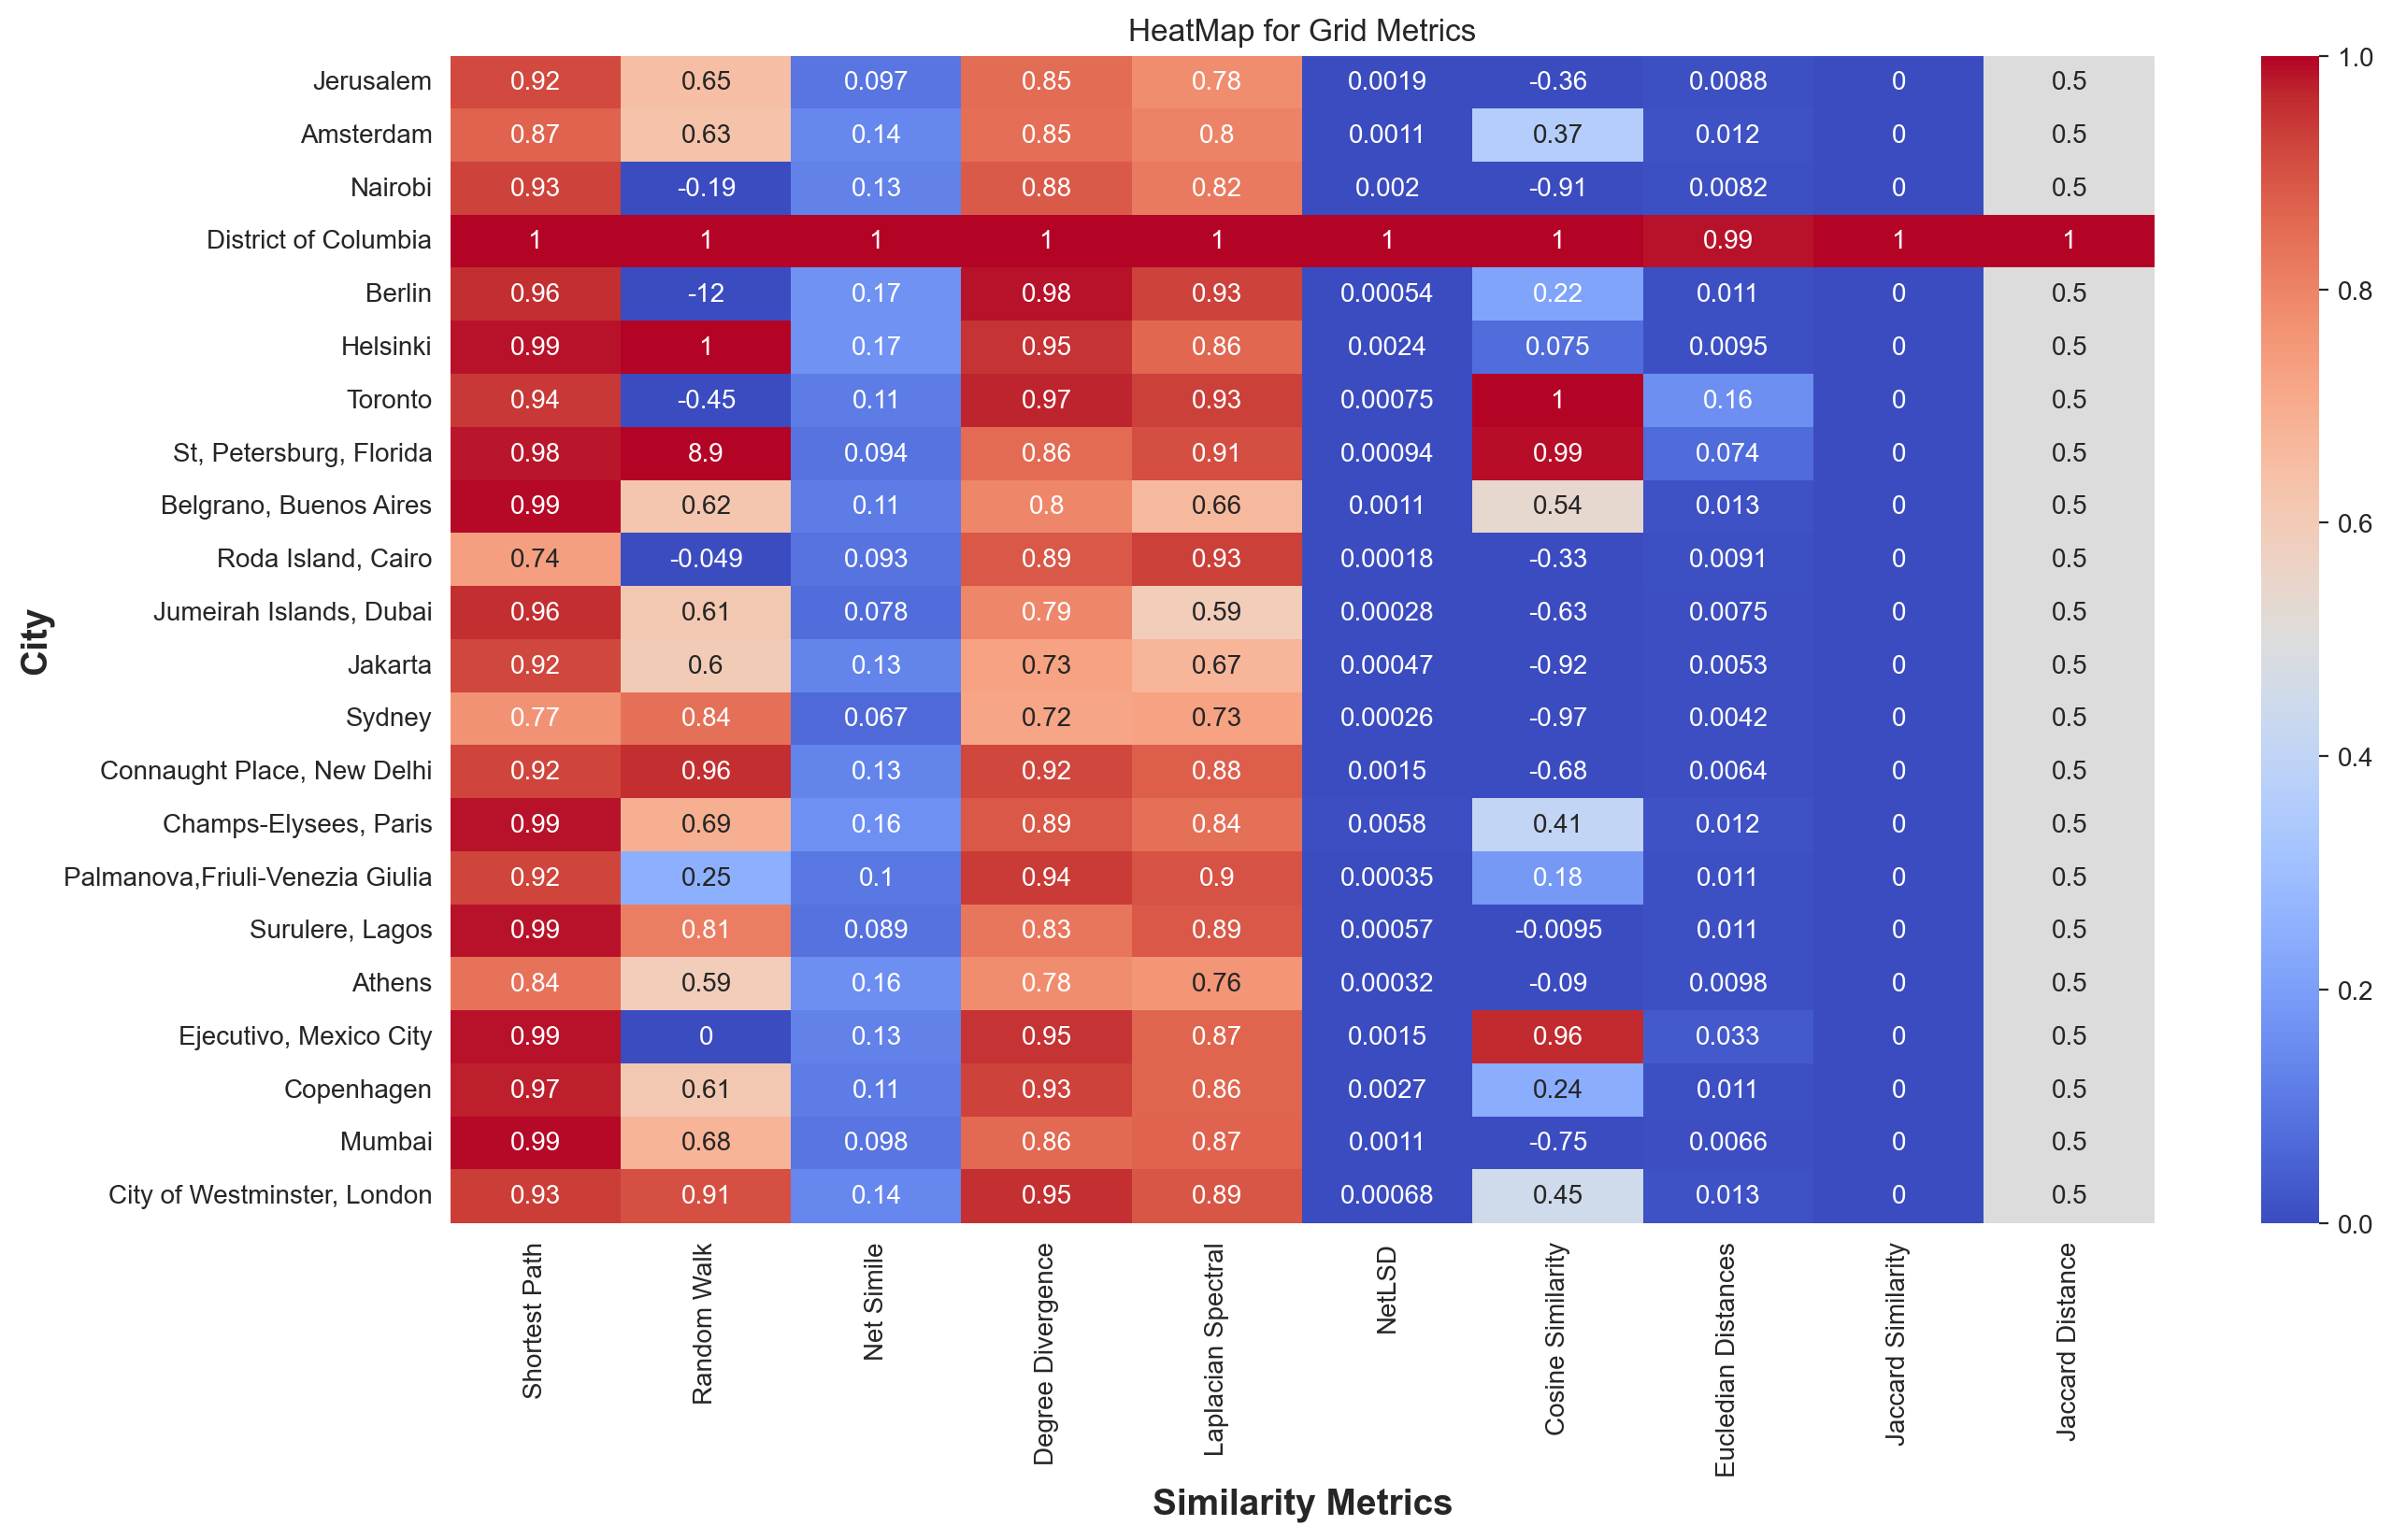
\includegraphics[width=0.85\textwidth,center]{picture/Grid/gridheatmap.png}
\caption[Heatmap showing the correlations for Grid Road Networks]{Heatmap showing the correlations between the road networks when the road network: District of Columbia (USA) was used as the reference network.}
\label{fig:Heatmap showing the correlations for Grid Road Networks}
\end{figure}

Dendrograms only tell us a little bit about the similarities of road networks based on the clusters generated, which is a major challenge when using them to visualize hierarchical clustering. The dendrogram shows a very different picture, with some road networks being grouped in different ways (see how the distribution of the road networks are mixed). For example, the clusters of Ejecutivo, Toronto, and the District of Columbia (USA) are later combined with the cluster of St. Petersburg, Florida, which is considered to be among the most similar to the reference network based on the similarity scores in figure \ref{fig:Heatmap showing the correlations for Grid Road Networks}. The dendrogram results are not suitable for interpreting the similarity results because they are not intuitive. Further analysis or another method of visualizing the results of similar scores is recommended in order to identify groups of clusters with similar road networks.

The pairwise Kendall-Tau distance between each pair of methods is calculated first, followed by a complete-linkage hierarchical clustering which then generates a dendrogram with many small clusters, which provides insight into which groups of methods are closely correlated.

\begin{figure}[!ht]
\centering
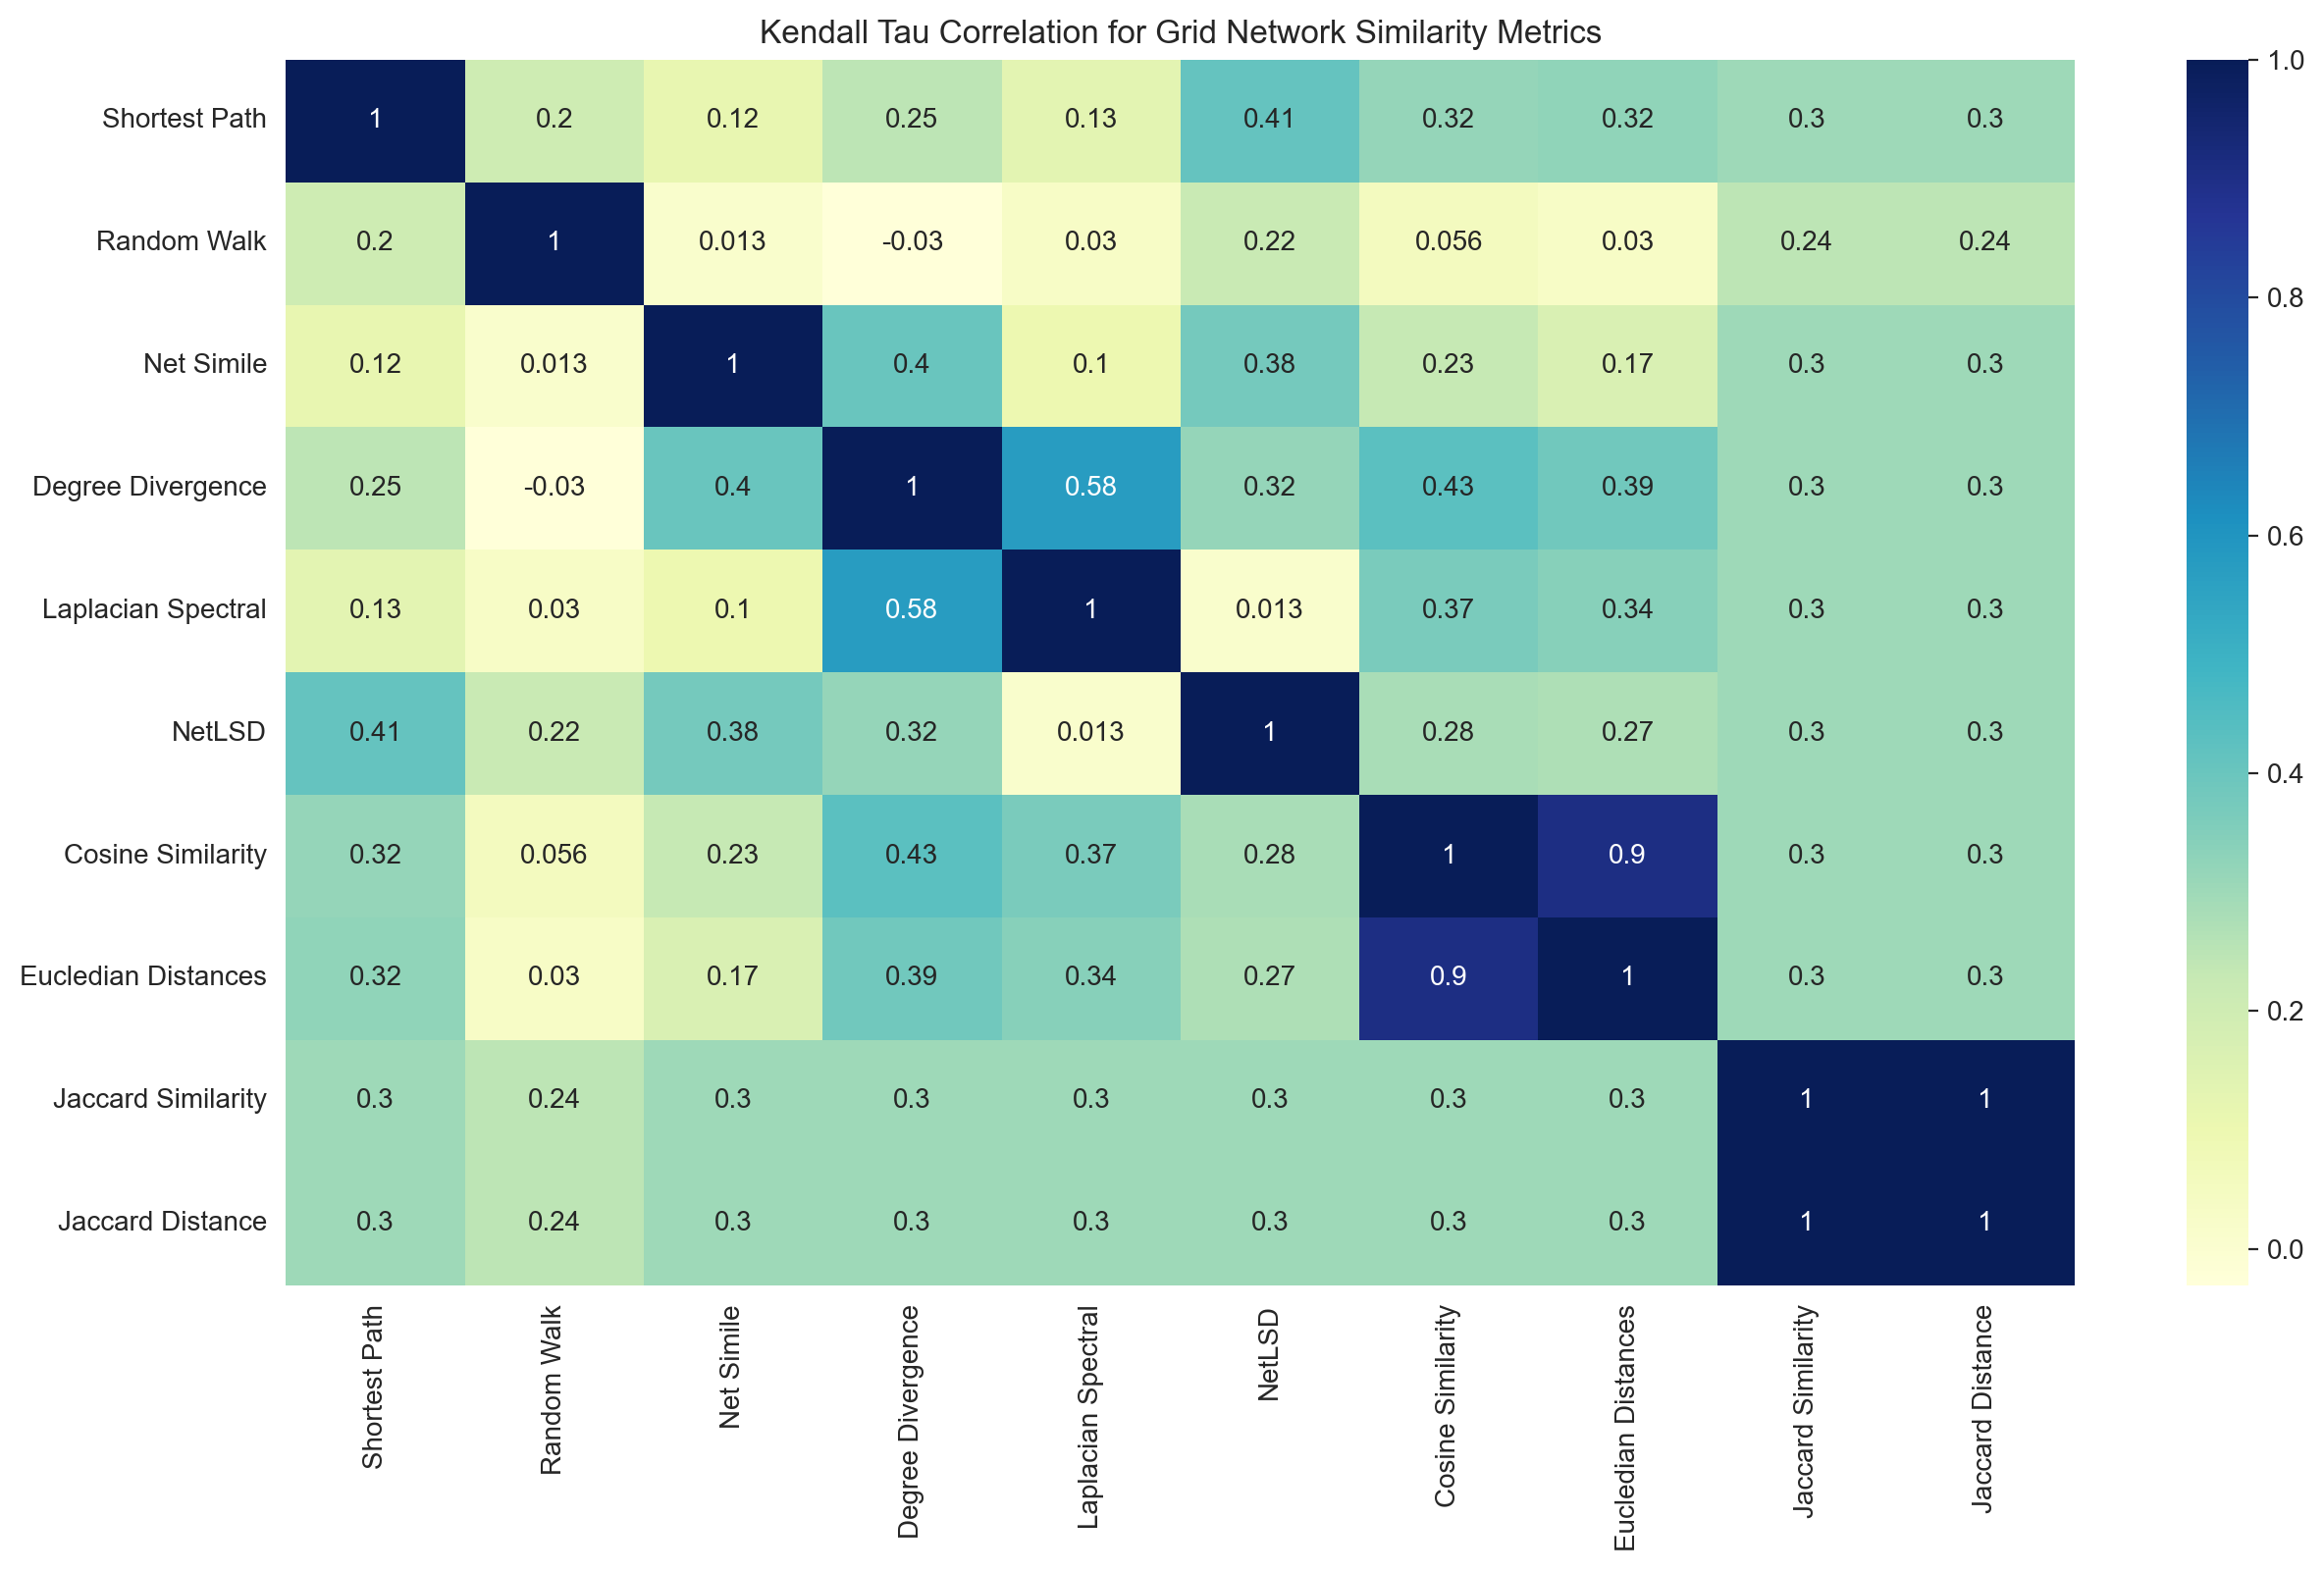
\includegraphics[width=0.85\textwidth,center]{picture/Grid/grid2.png}
\caption[Heatmap showing Kendall-Tau correlations between the road network similarity methods for Grid Road Networks]{Heatmap showing Kendall-Tau correlations between the road network similarity methods when the road network: District of Columbia (USA) was used as the reference network.}
\label{fig:network ranking grid}
\end{figure}

Each square depicts the relationship of the variables on each axis. Correlation values range from 0 to 1. Values close to zero indicate that the two variables do not have a linear relationship. The closer the correlation is to one, the more positively correlated they are; that is, as one rises, so does the other, and the closer the correlation is to one, the stronger the relationship. A correlation near zero is similar, but instead of both variables increasing, one variable decreases while the other increases. Because most squares perfectly correlate each variable to itself, the diagonals are all 1 or have dark blue color. For the other squares, the larger the number and the darker the color, the stronger the correlation between the two variables. The plot is also symmetrical about the diagonal because the same two variables are paired together in those squares.

Figure \ref{fig:network ranking grid} depicts the Kendall-Tau distances between the scores generated by the various methods when comparing road networks similar to the reference network with a Grid pattern. When both the Jaccard Distance and the Jaccard Similarity are used, the results show a one-to-one positive correlation. This is understandable given that the Jaccard Distance is thought to be complementary to the Jaccard Similarity, which is calculated by subtracting the Jaccard coefficient from 1. The methods cosine similarity and euclidean distance behave similarly, with a correlation of 0.9. Both methods are vector-based and operate at the micro level, as shown in table \ref{tab:Road Network Similarity Methods}. This means that either of the two methods could be used to calculate vector-based similarity on road networks at the Micro-level. The other methods, on the other hand, have a much weaker correlation because the level of the network they operate on and the type of comparison they use are different.Following that, the methods are clustered using complete linkage hierarchical clustering on pairwise Kendall Tau distances, as one of the goals of this approach is to determine whether certain network similarity methods are associated with each other. The dendrogram results are shown in the appendix.

\section{Radial Road Network Similarity Analysis}

For the Radial road similarity analysis, the Connaught Place in New Delhi road network is chosen as the reference network, and the methods are used to compare the other networks to the reference network and generate a numerical similarity score. The networks are then organized into hierarchical clusters. Figure \ref{fig:Hierarchical Clustering Dendrogram for Radial Road Networking Similarity} shows the results of this analysis.

\begin{figure}[!ht]
\centering
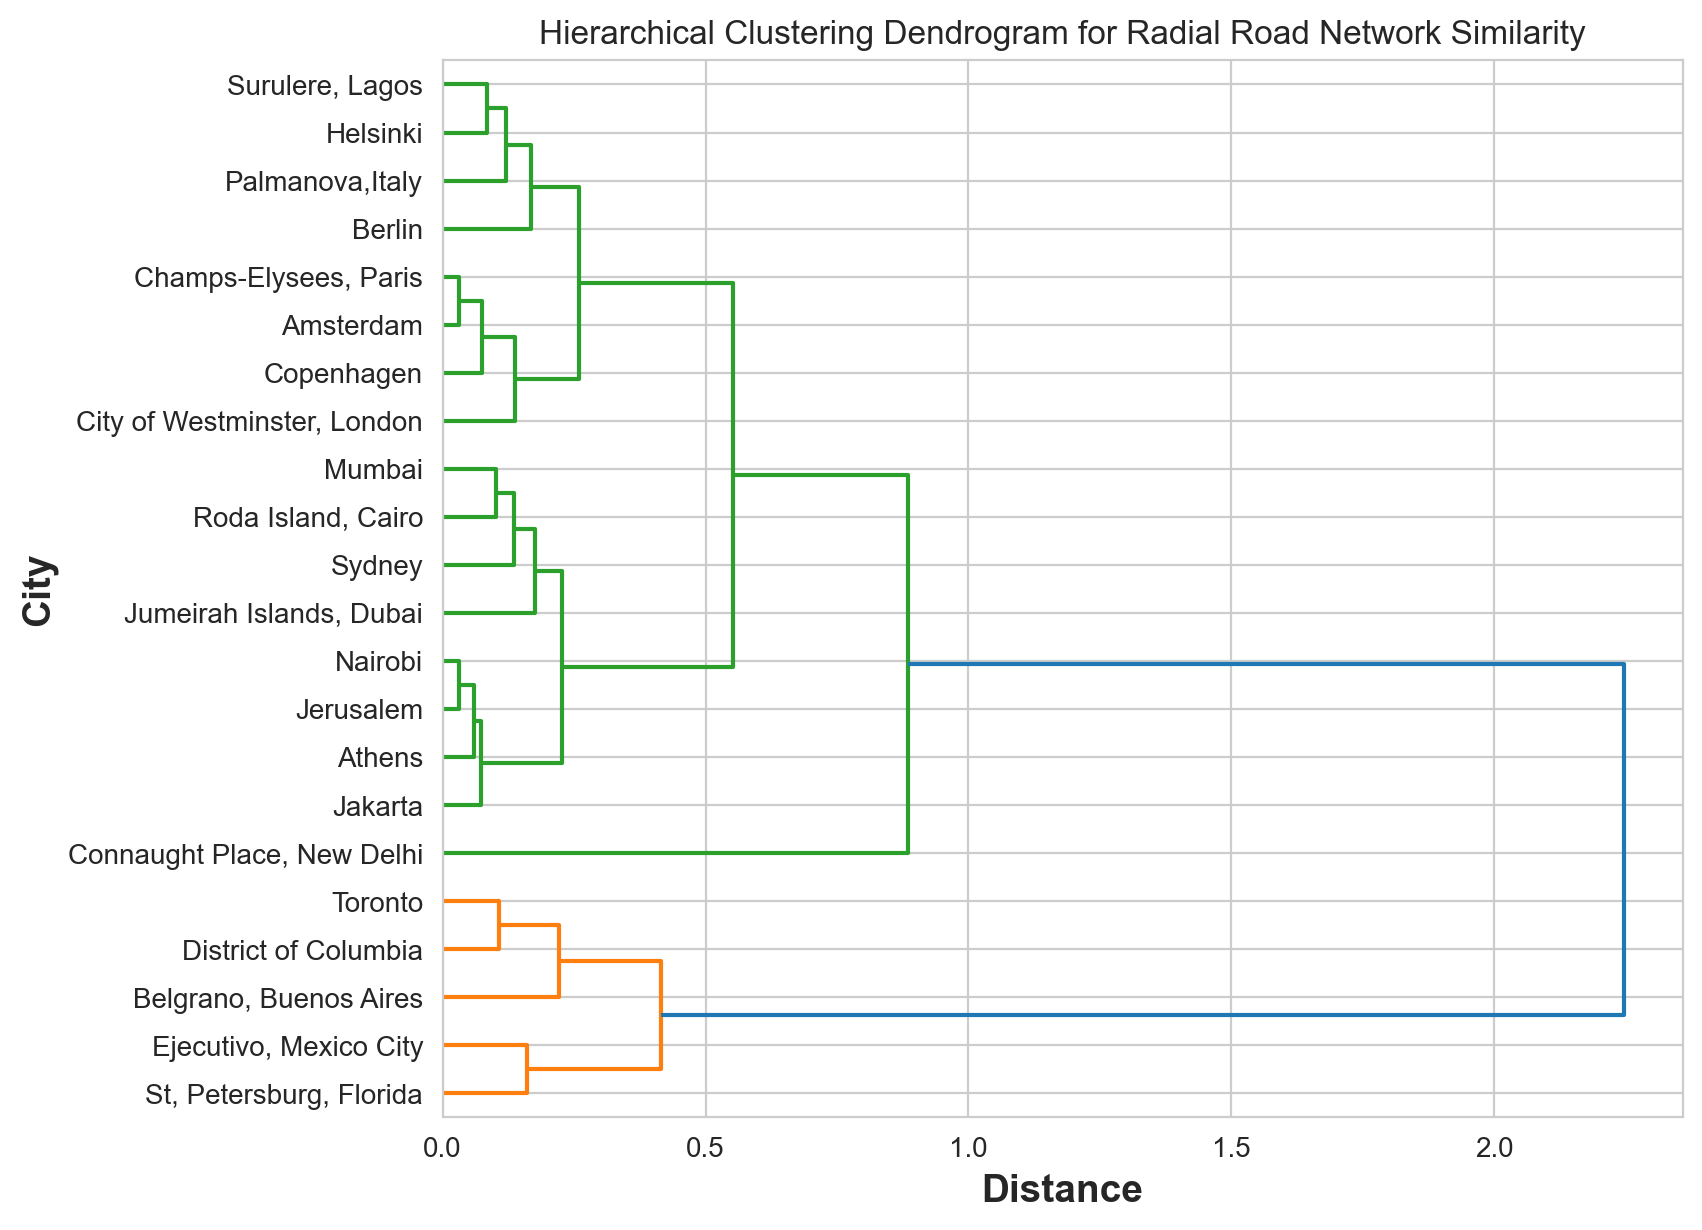
\includegraphics[width=0.75\textwidth,center]{picture/Radial/radial_dendrogram2.png}
\caption[Hierarchical Clustering Dendrogram for Radial Road Networking Similarity]{Hierarchical Clustering Dendrogram for Radial Road Networking Similarity}
\label{fig:Hierarchical Clustering Dendrogram for Radial Road Networking Similarity}
\end{figure}

The dendrogram obtained from the cluster analysis is shown in figure \ref{fig:Hierarchical Clustering Dendrogram for Radial Road Networking Similarity}. The two criteria described in Section 4.1 are used to interpret the dendrogram. The structure of the dendrogram reveals two major clusters (Green and Orange) for the first criteria. There are no road networks in the green cluster that are close to the reference network. All Road network patterns identified using Grid network analysis that have the most pronounced grid-like structure, on the other hand, are clustered together (Orange Cluster). Using the second criterion, the road networks of the cities Champs-Elysees, Paris, and Amsterdam, Netherlands are said to be clustered first because they have the cluster with the relatively shortest distance, followed by the cities Nairobi and Jerusalem because they are the most similar to any other cluster of road networks.
In comparison to the Grid Network Analysis, the majority of the road networks with similar patterns to the reference network with a radial like structure are clustered together (green) and have shorter distances, whereas the road networks with less similar patterns are clustered separately (Orange Cluster). This is to be expected because it is possible to identify the characteristics of each cluster and why certain clusters are grouped together by cross-checking with the similarity scores for each method included in the heatmap in figure \ref{fig:Heatmap showing the correlations for Radial Road Networks} and the structure of the graphs in figure \ref{fig:roadnetworkgraphs}.

\begin{figure}[!ht]
\centering
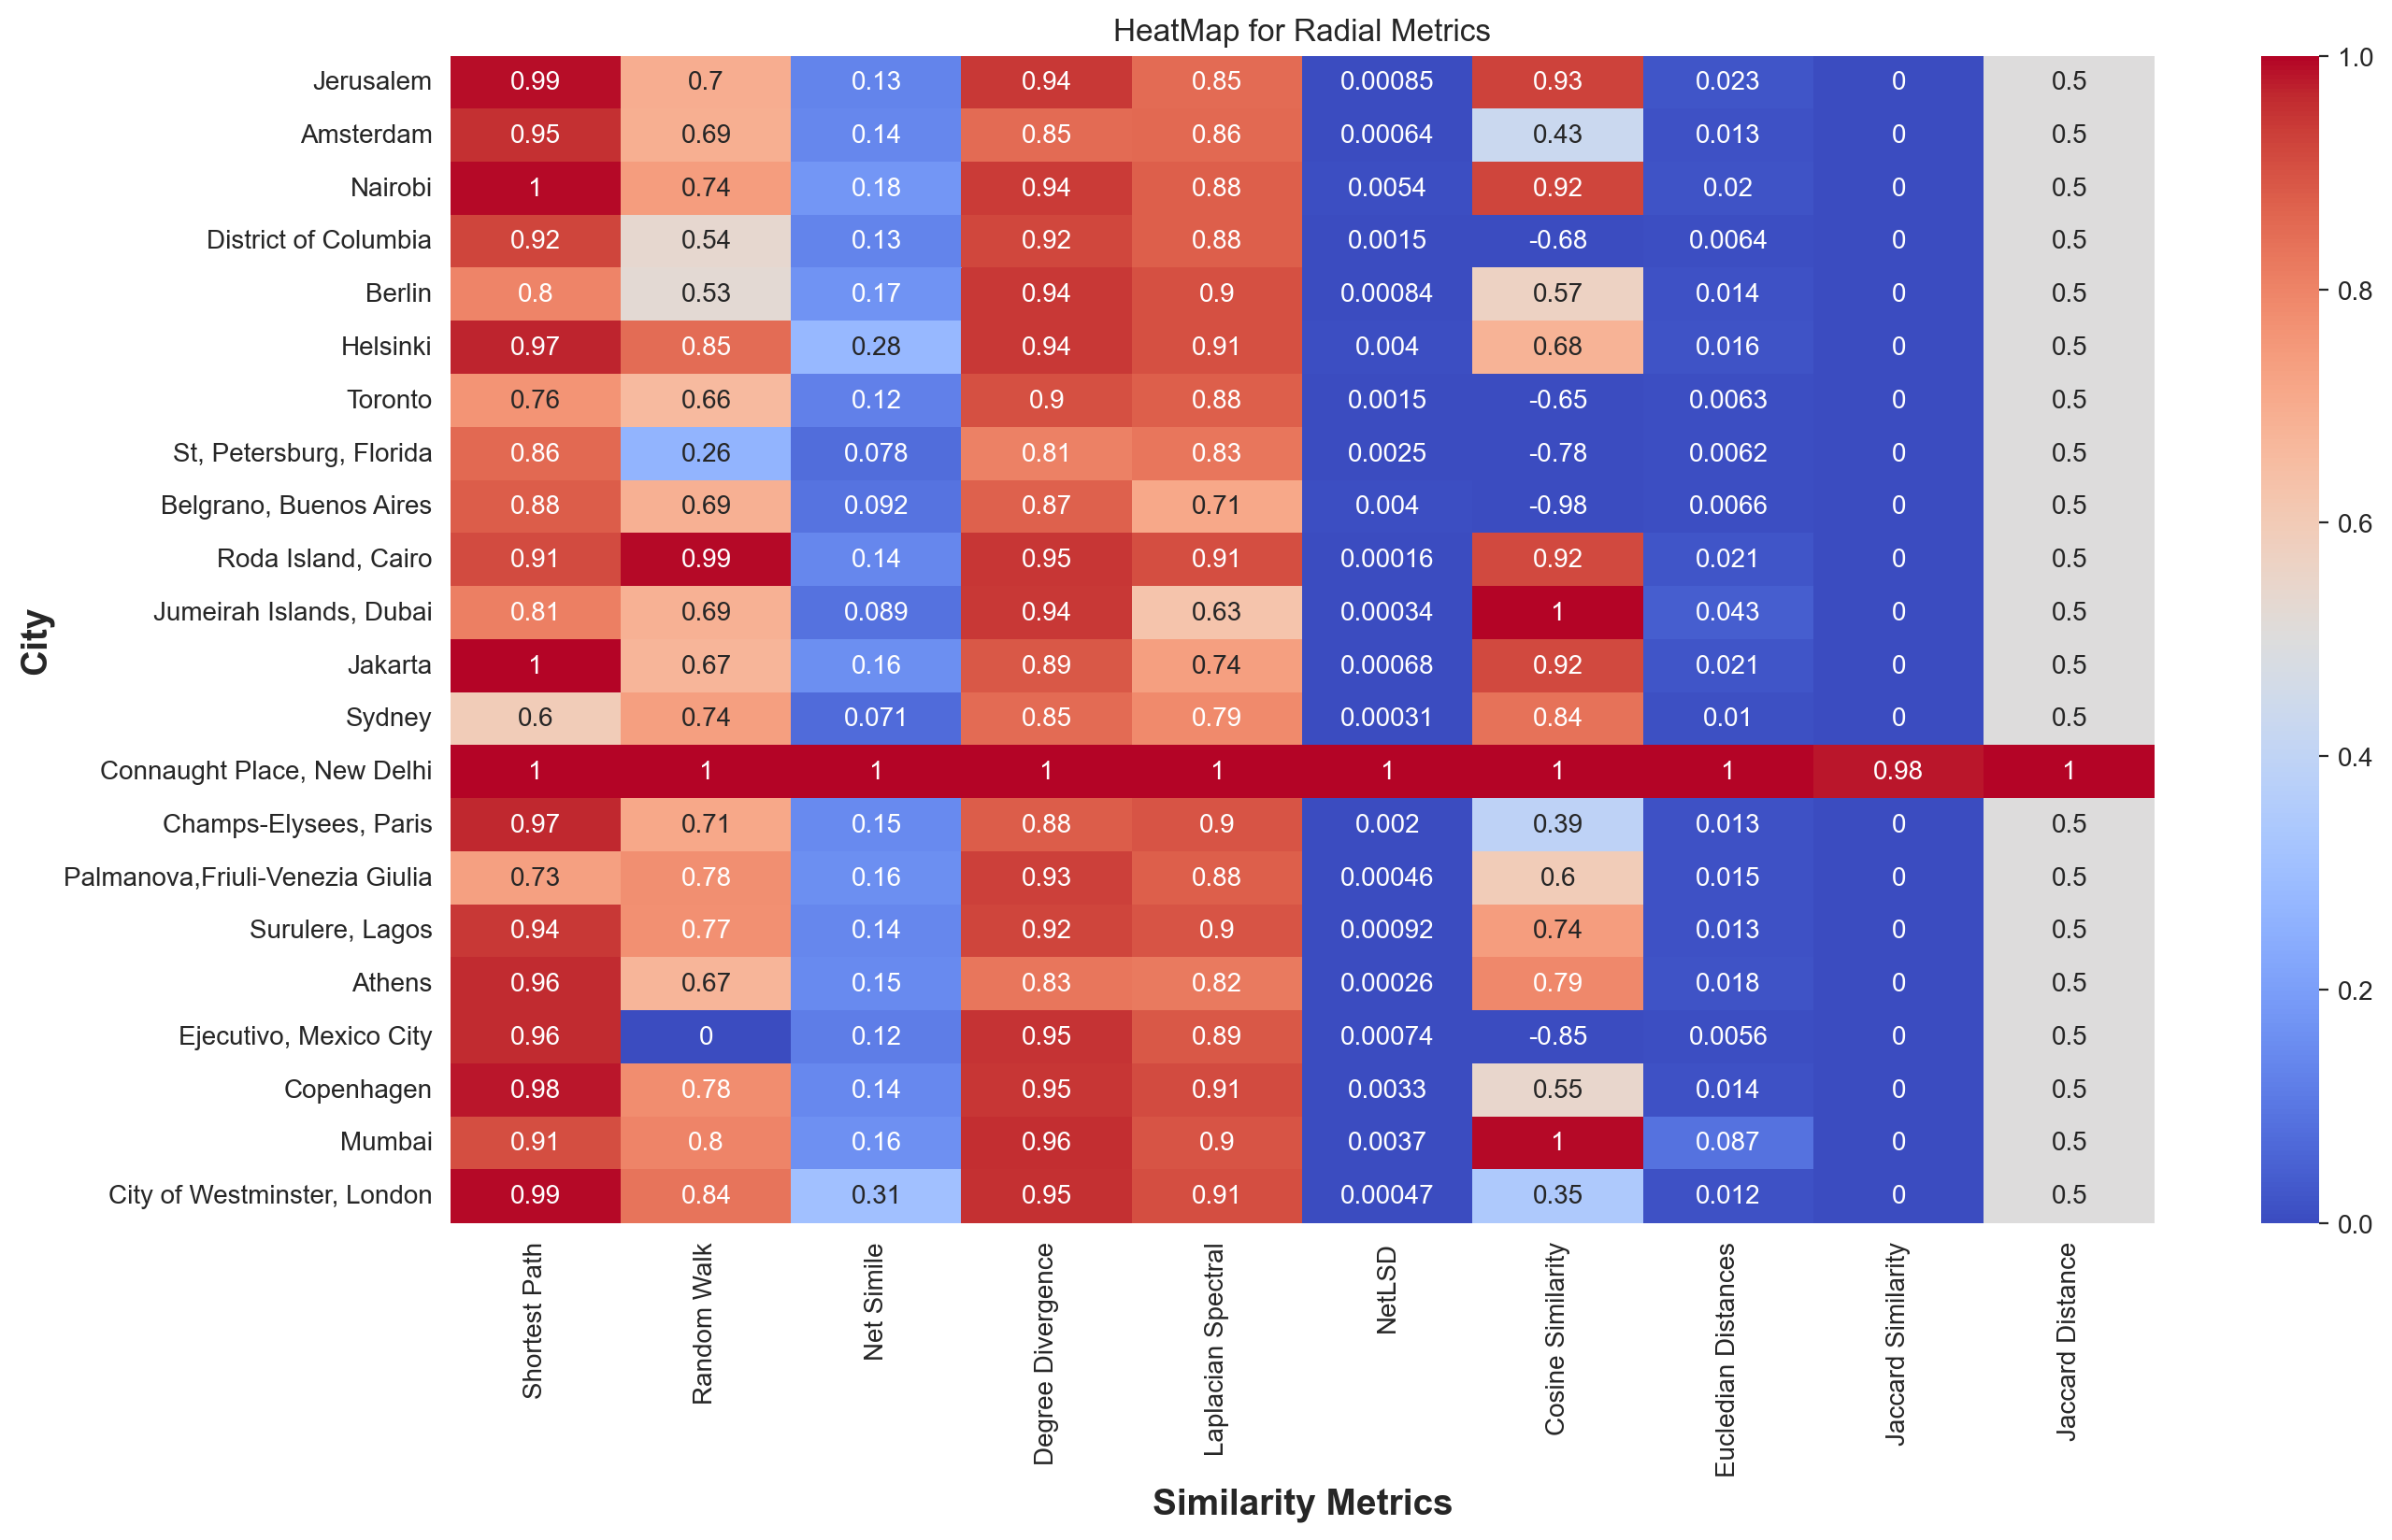
\includegraphics[width=0.85\textwidth,center]{picture/Radial/radialheatmap.png}
\caption[Heatmap showing the correlations for Radial Road Networks]{Heatmap showing the correlations between the road networks when the road network: Connaught Place (New Delhi) was used as the reference network.}
\label{fig:Heatmap showing the correlations for Radial Road Networks}
\end{figure}

As previously stated, additional analysis or another method to visualize the results of similar scores is recommended because the dendrogram results are not intuitive, making it unsuitable for interpreting the similarity results.

The pairwise Kendall-Tau distance between each pair of methods is calculated first, followed by a complete-linkage hierarchical clustering because it produces a dendrogram with many small clusters, which provides insight into which groups of methods are closely correlated.

\begin{figure}[!ht]
\centering
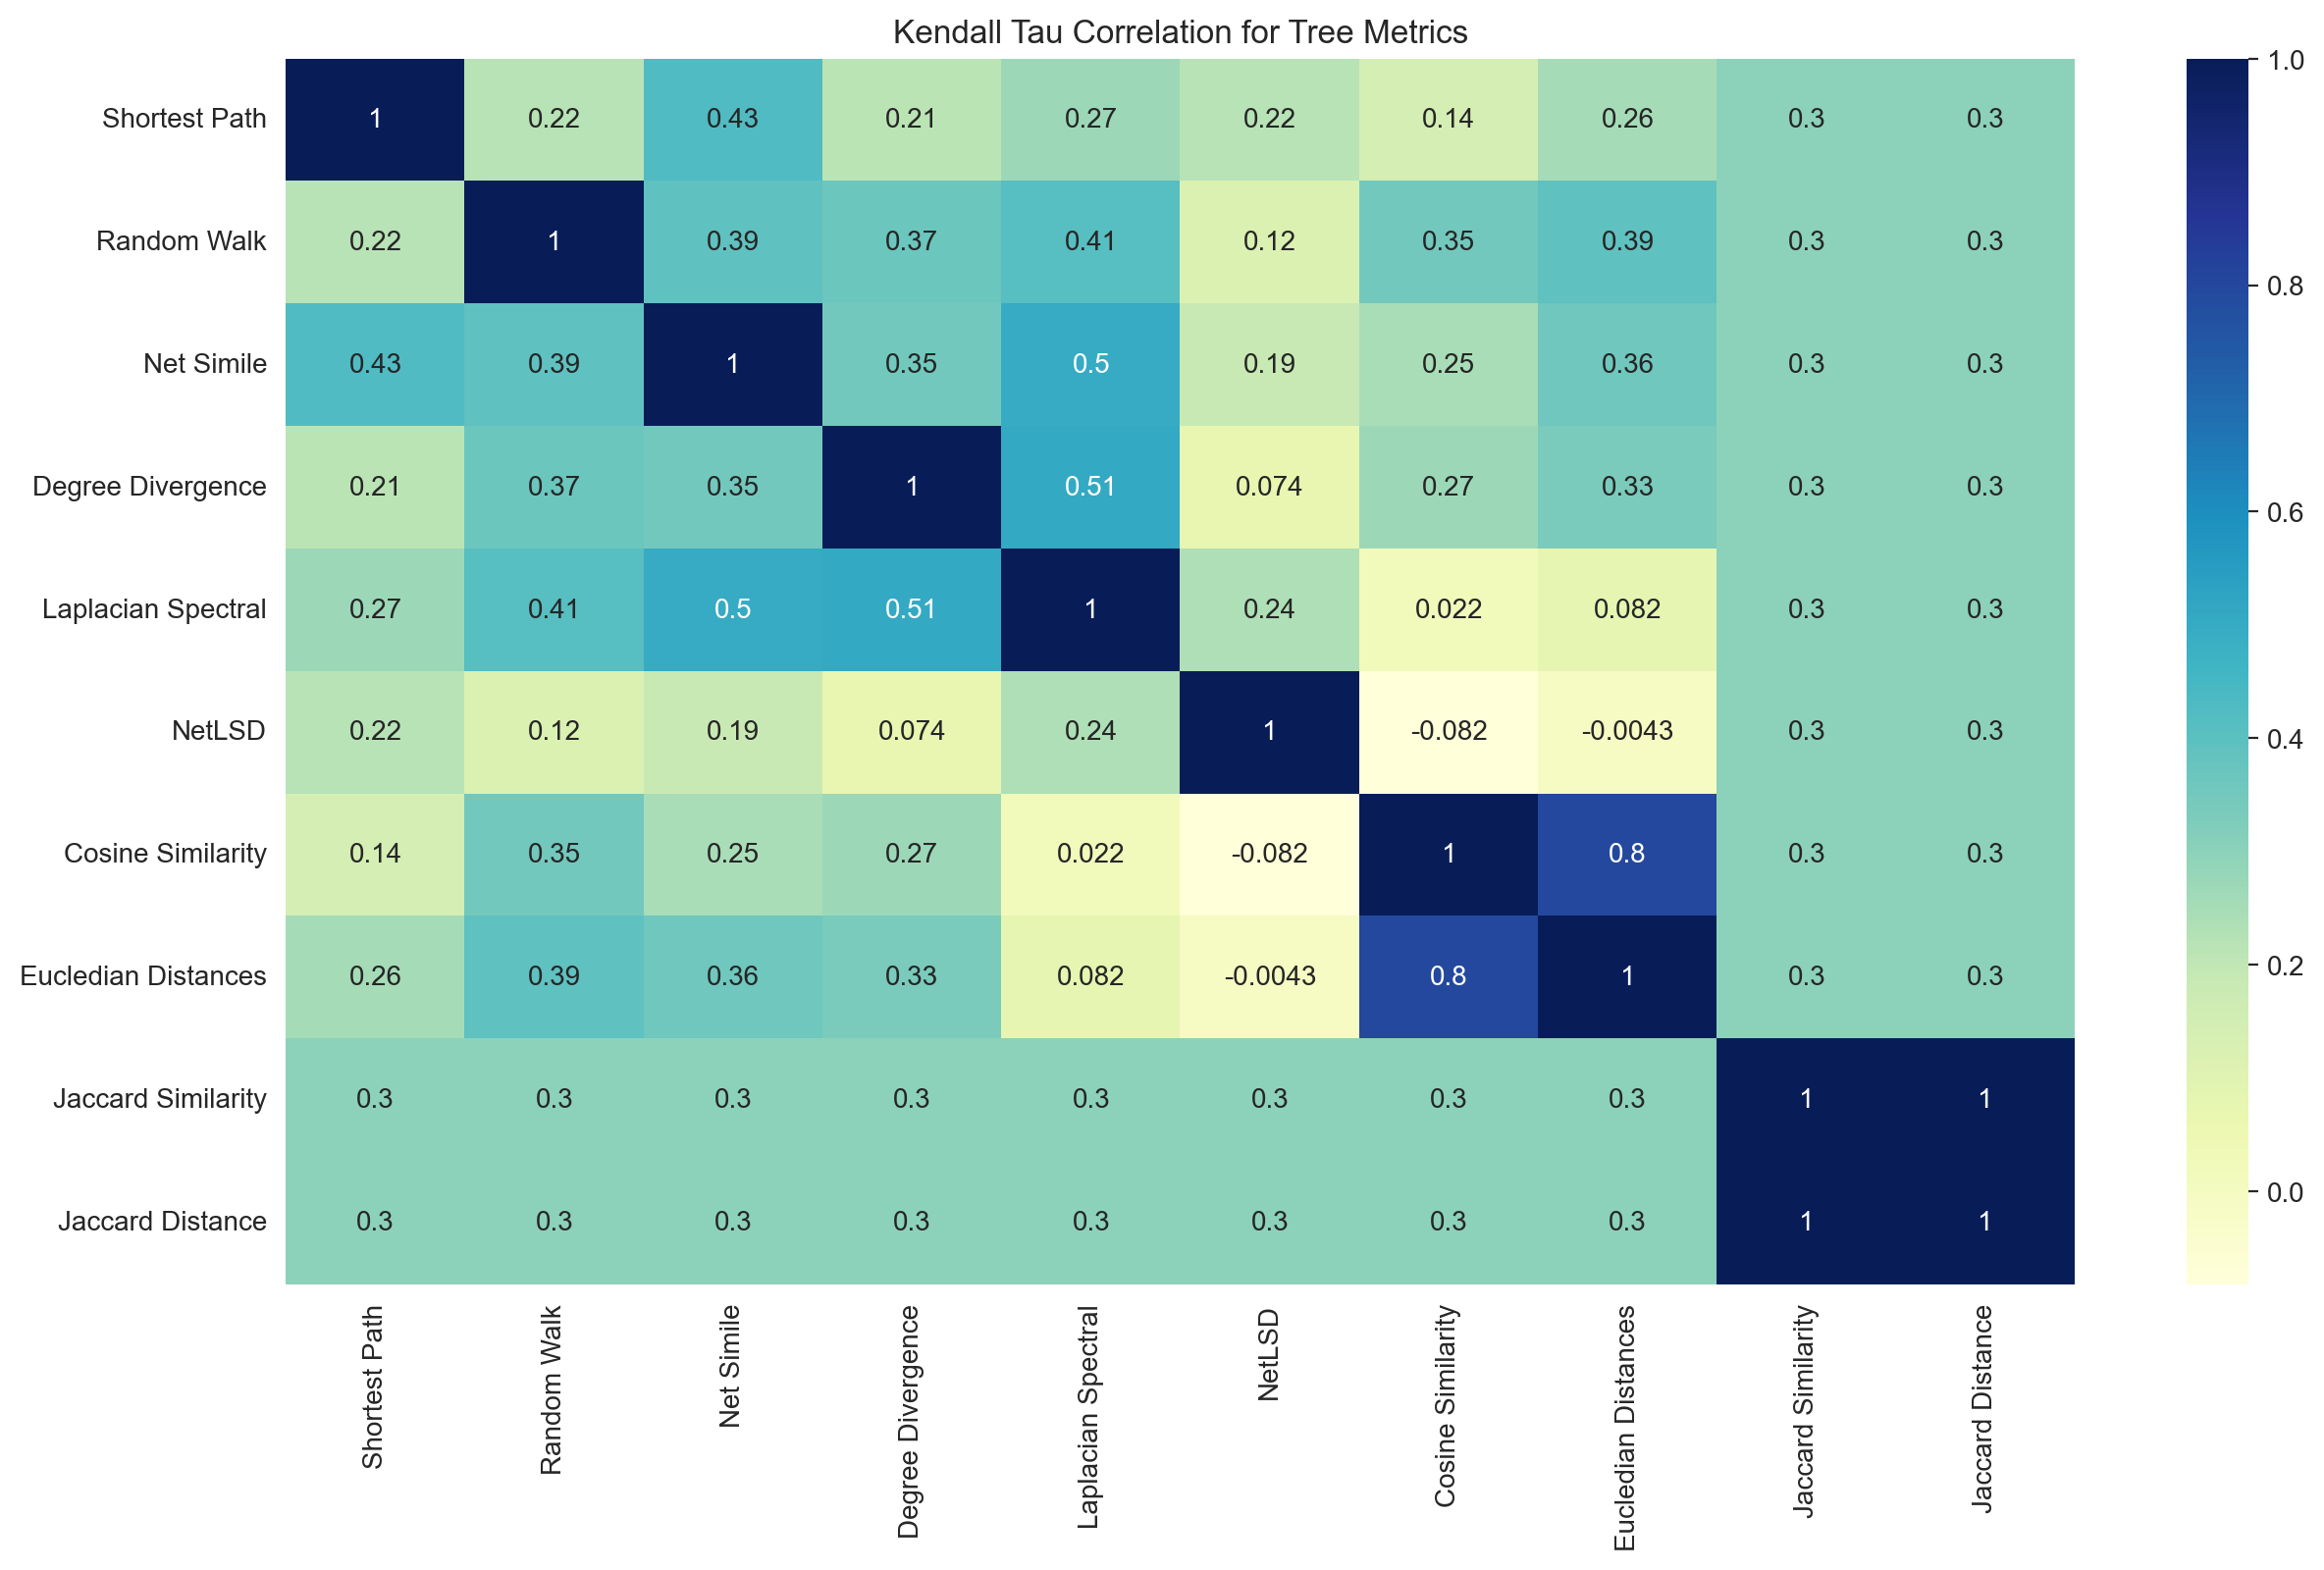
\includegraphics[width=0.85\textwidth,center]{picture/Radial/radial2.png}
\caption[Heatmap showing Kendall-Tau correlations between the road network similarity methods for Radial Road Networks]{Heatmap showing Kendall-Tau correlations between the road network similarity methods when the road network: District of Columbia was used as the reference network.}
\label{fig:network ranking radial}
\end{figure}

Figure \ref{fig:network ranking radial}. depicts the Kendall-Tau distances between the scores generated by the various methods when comparing road networks similar to the reference network with a Radial like structure. When both the Jaccard Distance and the Jaccard Similarity are used, the results show a one-to-one positive correlation. This is understandable given that the Jaccard Distance is thought to be complementary to the Jaccard Similarity, which is calculated by subtracting the Jaccard coefficient from 1. The methods cosine similarity and euclidean distance behave similarly, with a correlation of 0.8. Both methods are vector-based and operate at the micro level, as shown in table \ref{tab:Road Network Similarity Methods}. This means that either of the two methods could be used to calculate vector-based similarity on road networks at the micro-level. The other methods, on the other hand, have a much weaker correlation because the level of the network they operate on and the type of comparison they use are different.
Following that, the methods are clustered using complete linkage hierarchical clustering on pairwise Kendall Tau distances, as one of the goals of this approach is to determine whether certain network similarity methods are associated with each other. The dendrogram results are shown in the appendix.

\section{Tree Road Network Similarity Analysis}

For the Tree road similarity analysis, the City of Westminster in London is chosen as the reference network, and the methods are used to compare the other networks to the reference network and generate a numerical similarity score. The networks are then organized into hierarchical clusters. Figure \ref{fig:Hierarchical Clustering Dendrogram for Tree Road Networking Similarity} shows the results of this analysis.

\begin{figure}[!ht]
\centering
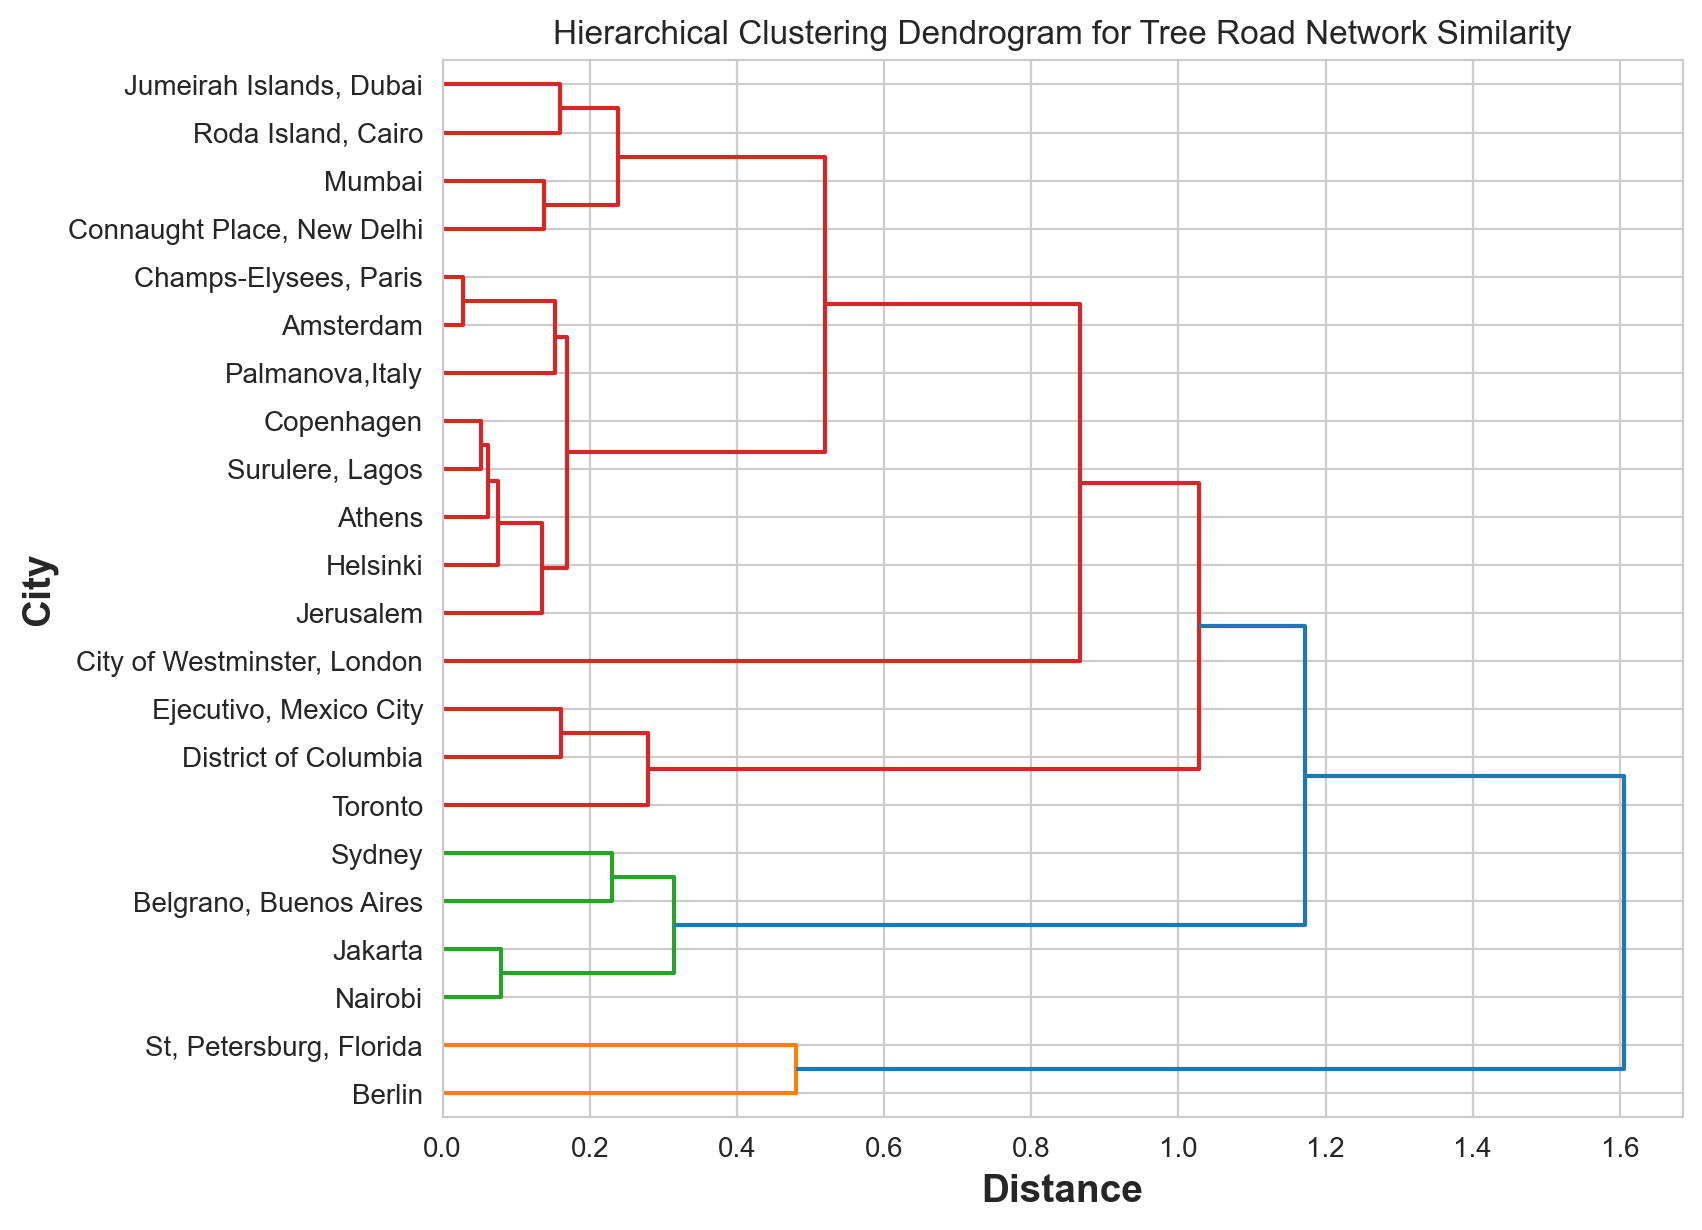
\includegraphics[width=0.75\textwidth,center]{picture/Tree/tree_dendrogram2.png}
\caption[Hierarchical Clustering Dendrogram for Tree Road Networking Similarity]{Hierarchical Clustering Dendrogram for Tree Road Networking Similarity}
\label{fig:Hierarchical Clustering Dendrogram for Tree Road Networking Similarity}
\end{figure}

The dendrogram obtained from the cluster analysis is shown in figure \ref{fig:Hierarchical Clustering Dendrogram for Tree Road Networking Similarity}. The two criteria described in Section 4.1 are used to interpret the dendrogram.

For the first criteria, the dendrogram structure reveals three major clusters (Red, Green, and Orange). Using the first criteria to interpret the generated clusters, however, fails because the dendrogram results are not intuitive because some clusters contained a mix of road networks with varying structures. For example, Berlin is in the same cluster as St. Petersburg, Florida. Furthermore, based on the heatmap similarity scores in figure \ref{fig:Heatmap showing the correlations for Tree Road Networks}, they are not expected to be in the same cluster, as is evident for other clusters. Using the second criterion, the road networks of the cities Champs-Elysees, Paris, and Amsterdam, Netherlands are said to be clustered first, as shown in figure \ref{fig:Hierarchical Clustering Dendrogram for Grid Road Networking Similarity} and \ref{fig:Hierarchical Clustering Dendrogram for Radial Road Networking Similarity} becoming a repetitive pattern, as they tend to have the cluster with the relatively shortest distance, followed by Copenhagen and Surulere, Lagos.

In comparison to the Grid and Radial Network Analysis, the road network: Mumbai, which is identified as the other only tree road network pattern in table \ref{tab:Selected Cities}, is located within the same cluster (red), but farther away from the reference road network. This is to be expected because we can tell why they are not grouped together by examining the characteristics of each cluster and cross-checking the similarity scores for each method included in the heatmap in figure \ref{fig:Heatmap showing the correlations for Tree Road Networks}.

\begin{figure}[!ht]
\centering
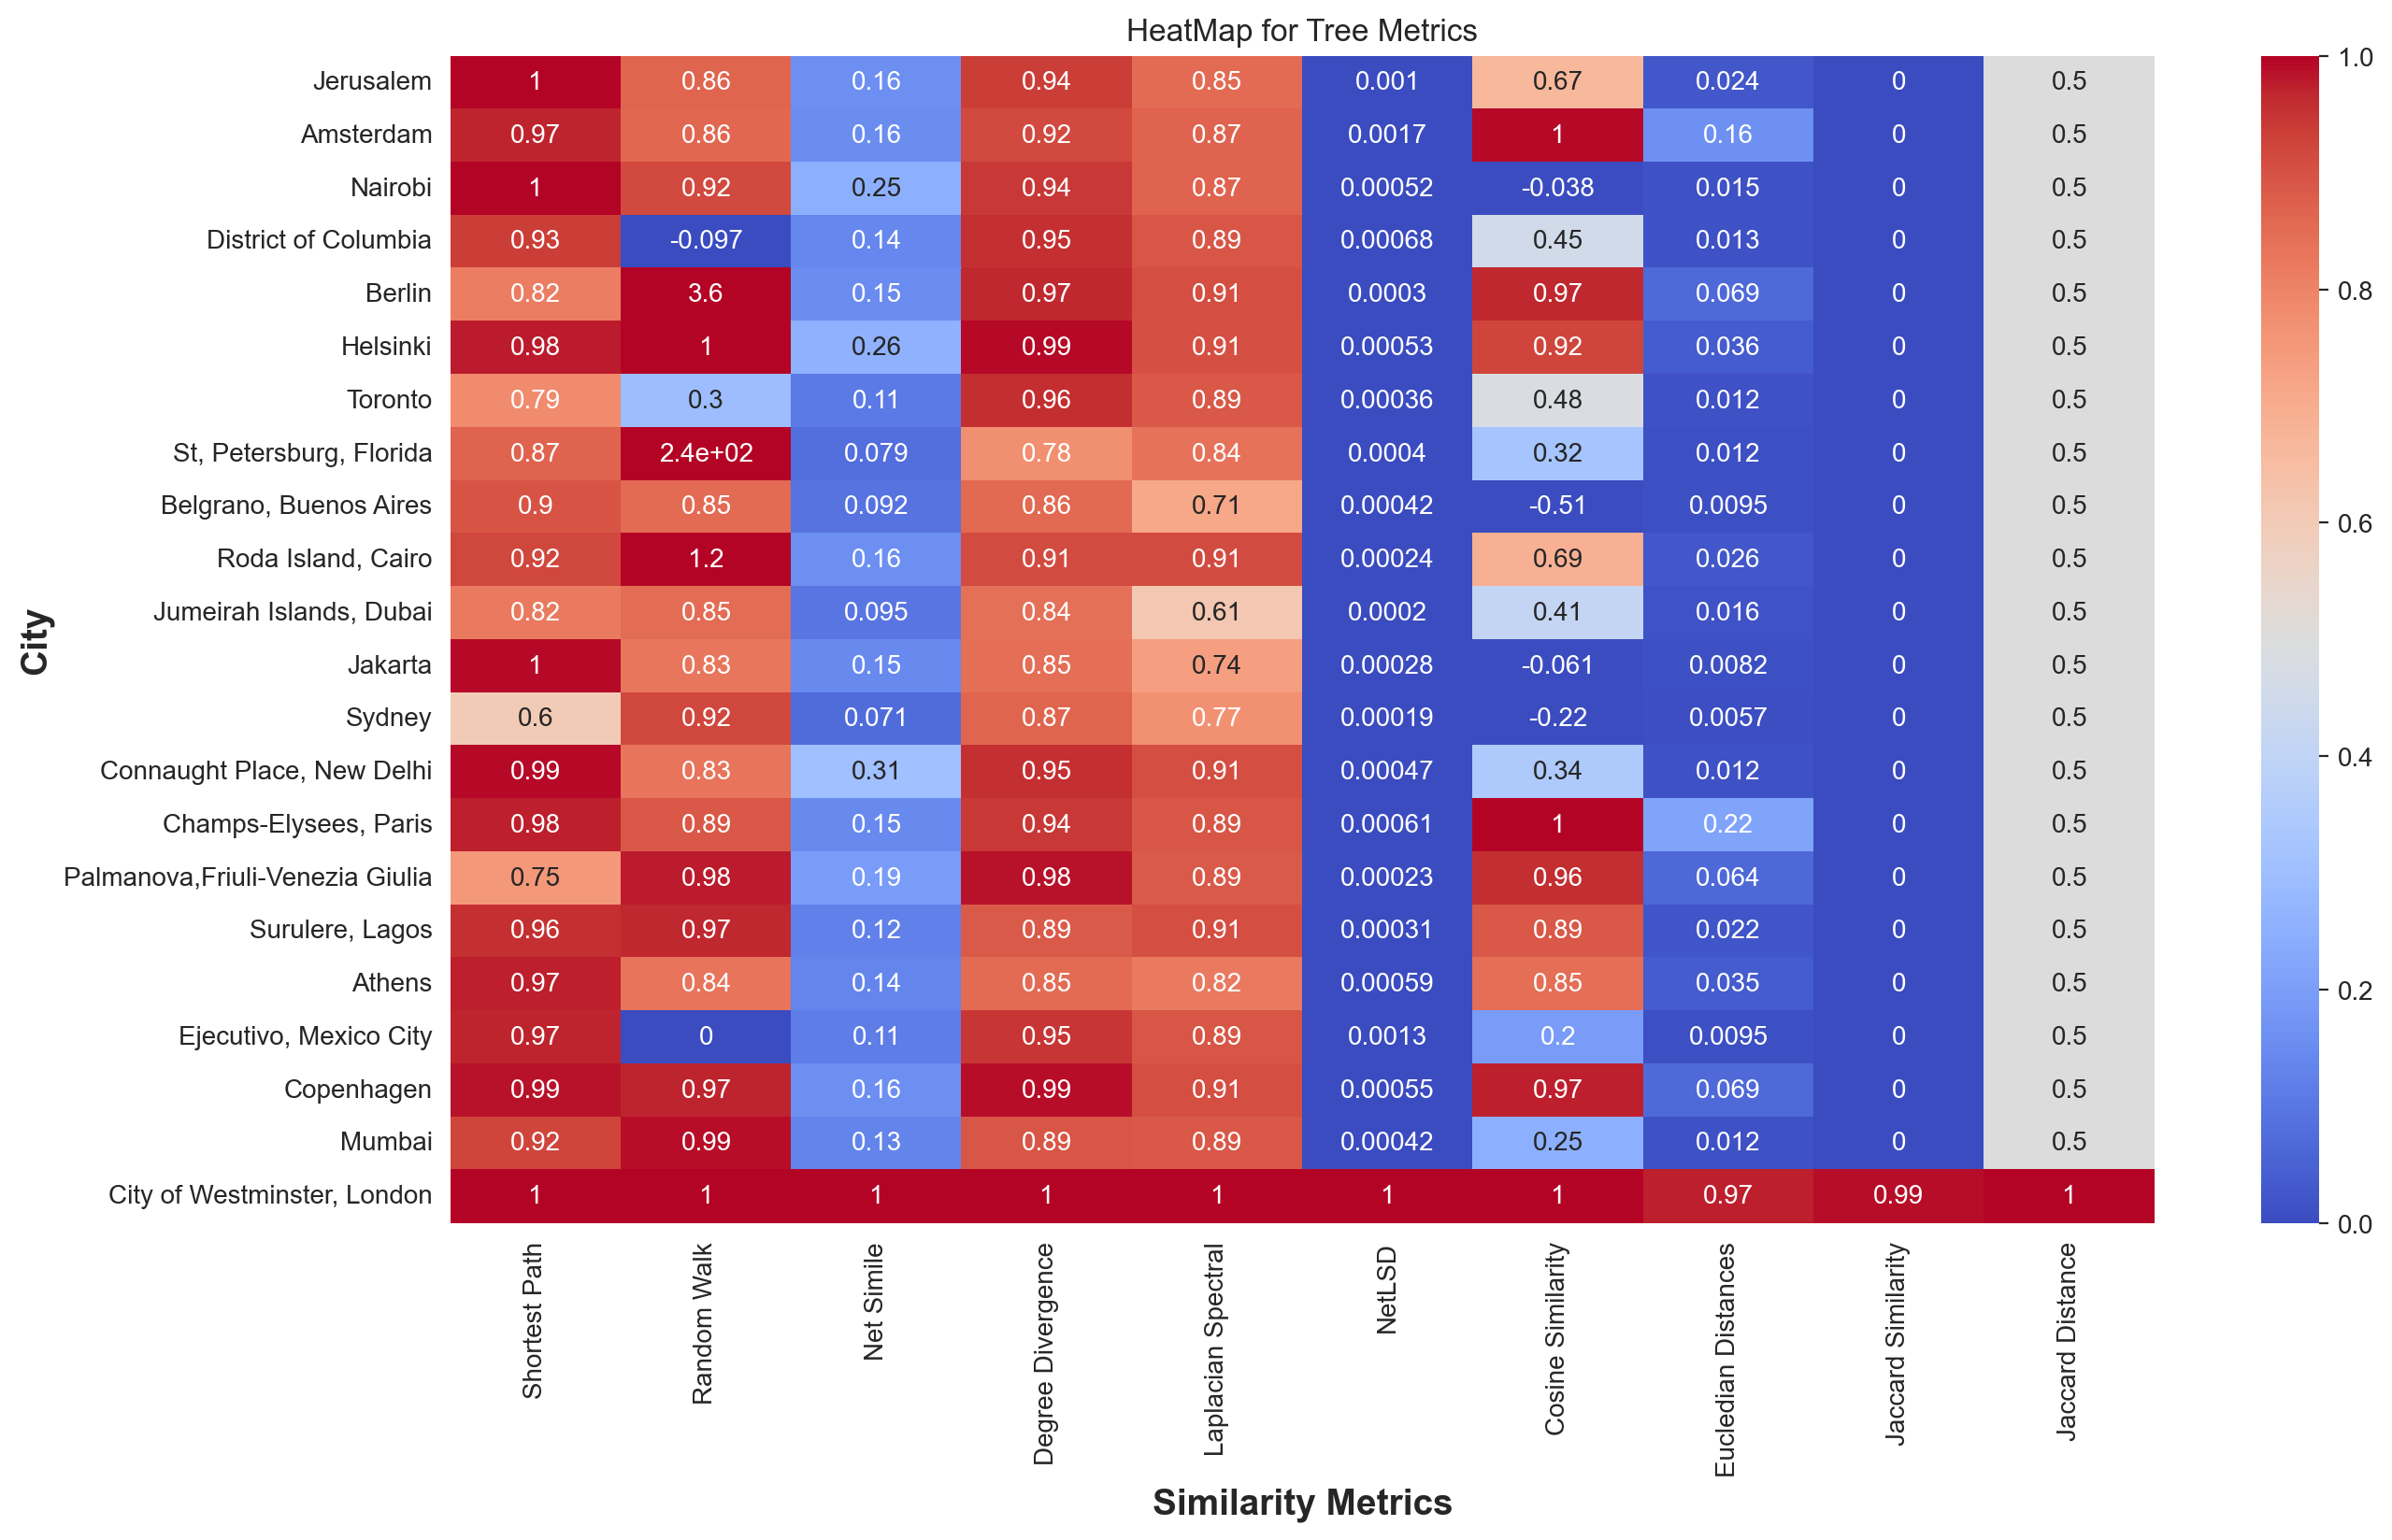
\includegraphics[width=0.85\textwidth,center]{picture/Tree/treeheatmap.png}
\caption[Heatmap showing the correlations for Tree Road Networks]{Heatmap showing the correlations between the road networks when the road network: City of Westminster, London was used as the reference network.}
\label{fig:Heatmap showing the correlations for Tree Road Networks}
\end{figure}

The pairwise Kendall-Tau distance between each pair of methods is calculated first, followed by a complete-linkage hierarchical clustering because it produces a dendrogram with many small clusters, which provides insight into which groups of methods are closely correlated.

\begin{figure}[!ht]
\centering
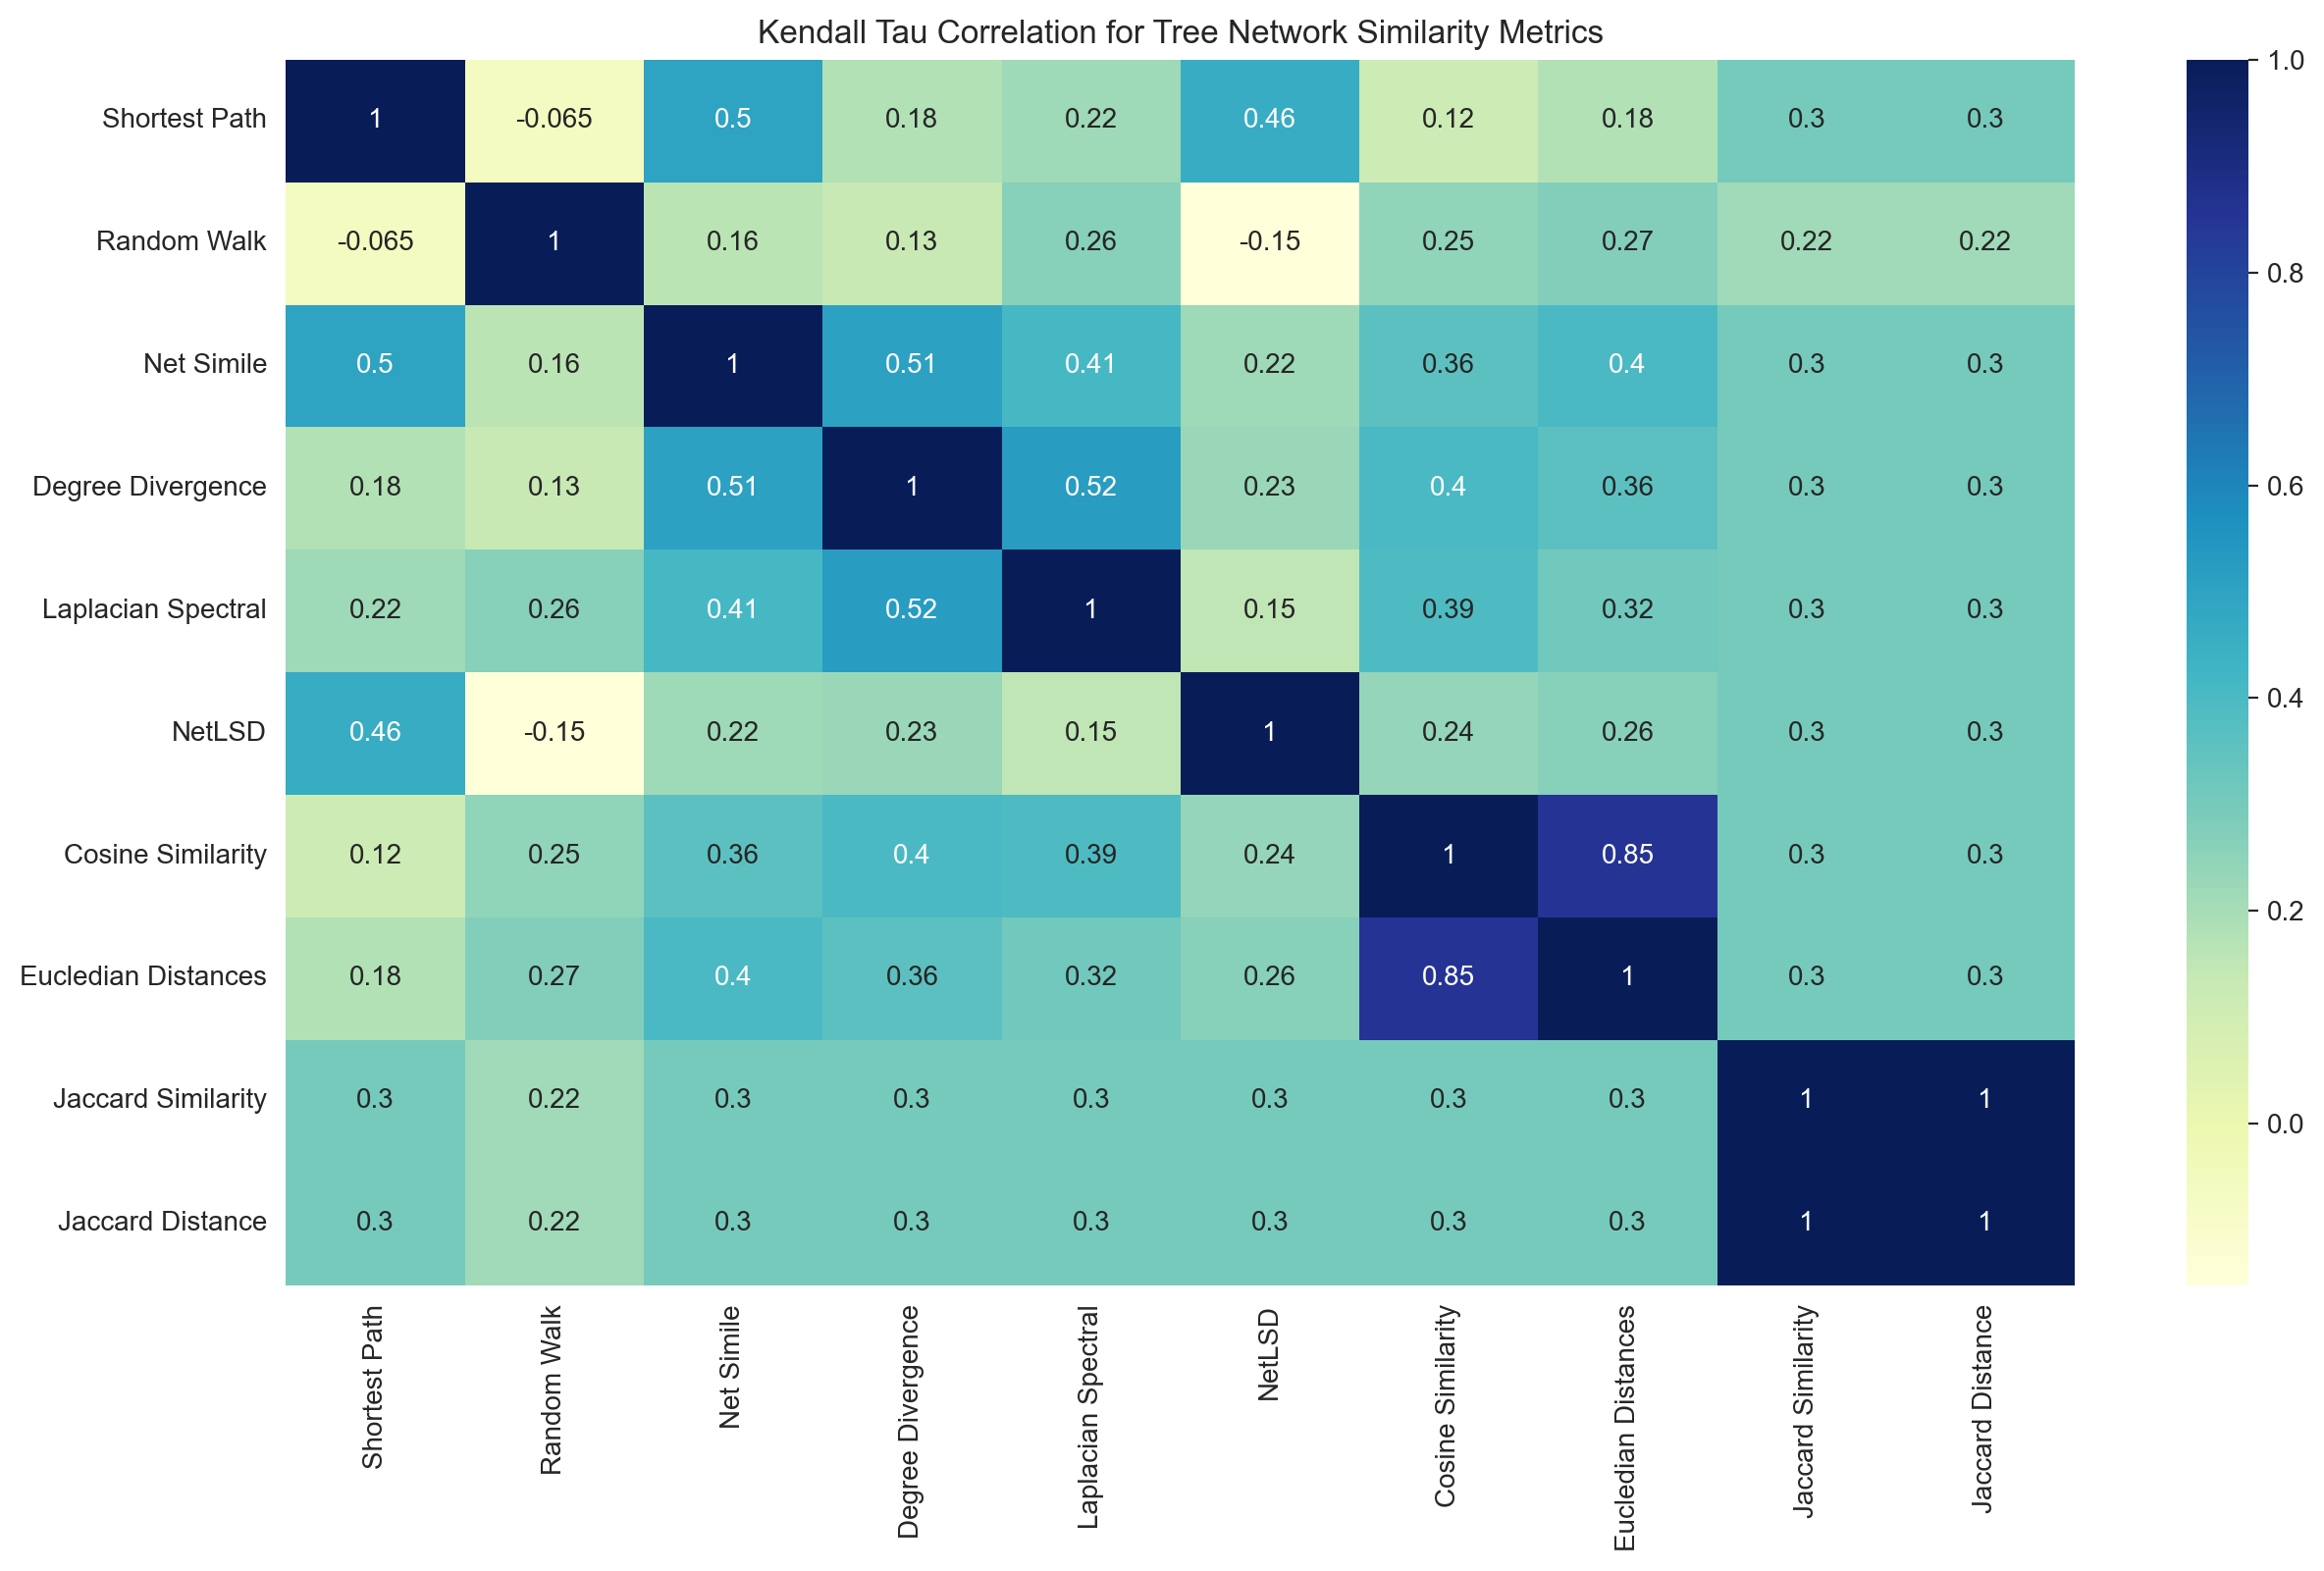
\includegraphics[width=0.85\textwidth,center]{picture/Tree/tree2.png}
\caption[Heatmap showing Kendall-Tau correlations between the road network similarity methods for Radial Road Networks]{Heatmap showing Kendall-Tau correlations between the road network similarity methods when the road network: City of Westminster (London) was used as the reference network.}
\label{fig:network ranking tree}
\end{figure}

Figure \ref{fig:network ranking tree} ranking tree depicts the Kendall-Tau distances between the scores generated by the various methods when comparing road networks similar to the reference network with a Tree-like structure. When both the Jaccard Distance and the Jaccard Similarity are used, the results show a one-to-one positive correlation. Again, this is understandable given that the Jaccard Distance is thought to be complementary to the Jaccard Similarity, which is calculated by subtracting the Jaccard coefficient from 1. The methods cosine similarity and euclidean distance also behave similarly, with a correlation of 0.85. Both methods are vector-based and operate at the micro-level, as shown in table \ref{tab:Road Network Similarity Methods}. This means that either of the two methods could be used to calculate vector-based similarity on road networks at the micro-level. The other methods, on the other hand, have a much weaker correlation because the level of the network they operate on and the type of comparison they use are different. The dendrogram results are shown in the appendix.

\section{Linear Road Network Similarity Analysis}

The road network in Sydney (Australia), was chosen as the reference network for the Linear road similarity analysis, and the methods were used to compare the other networks to the reference network and generate a numerical similarity score. The networks are then organized into hierarchical clusters. Figure \ref{fig:Hierarchical Clustering Dendrogram for Linear Road Networking Similarity} shows the results of this analysis.

\begin{figure}[!ht]
\centering
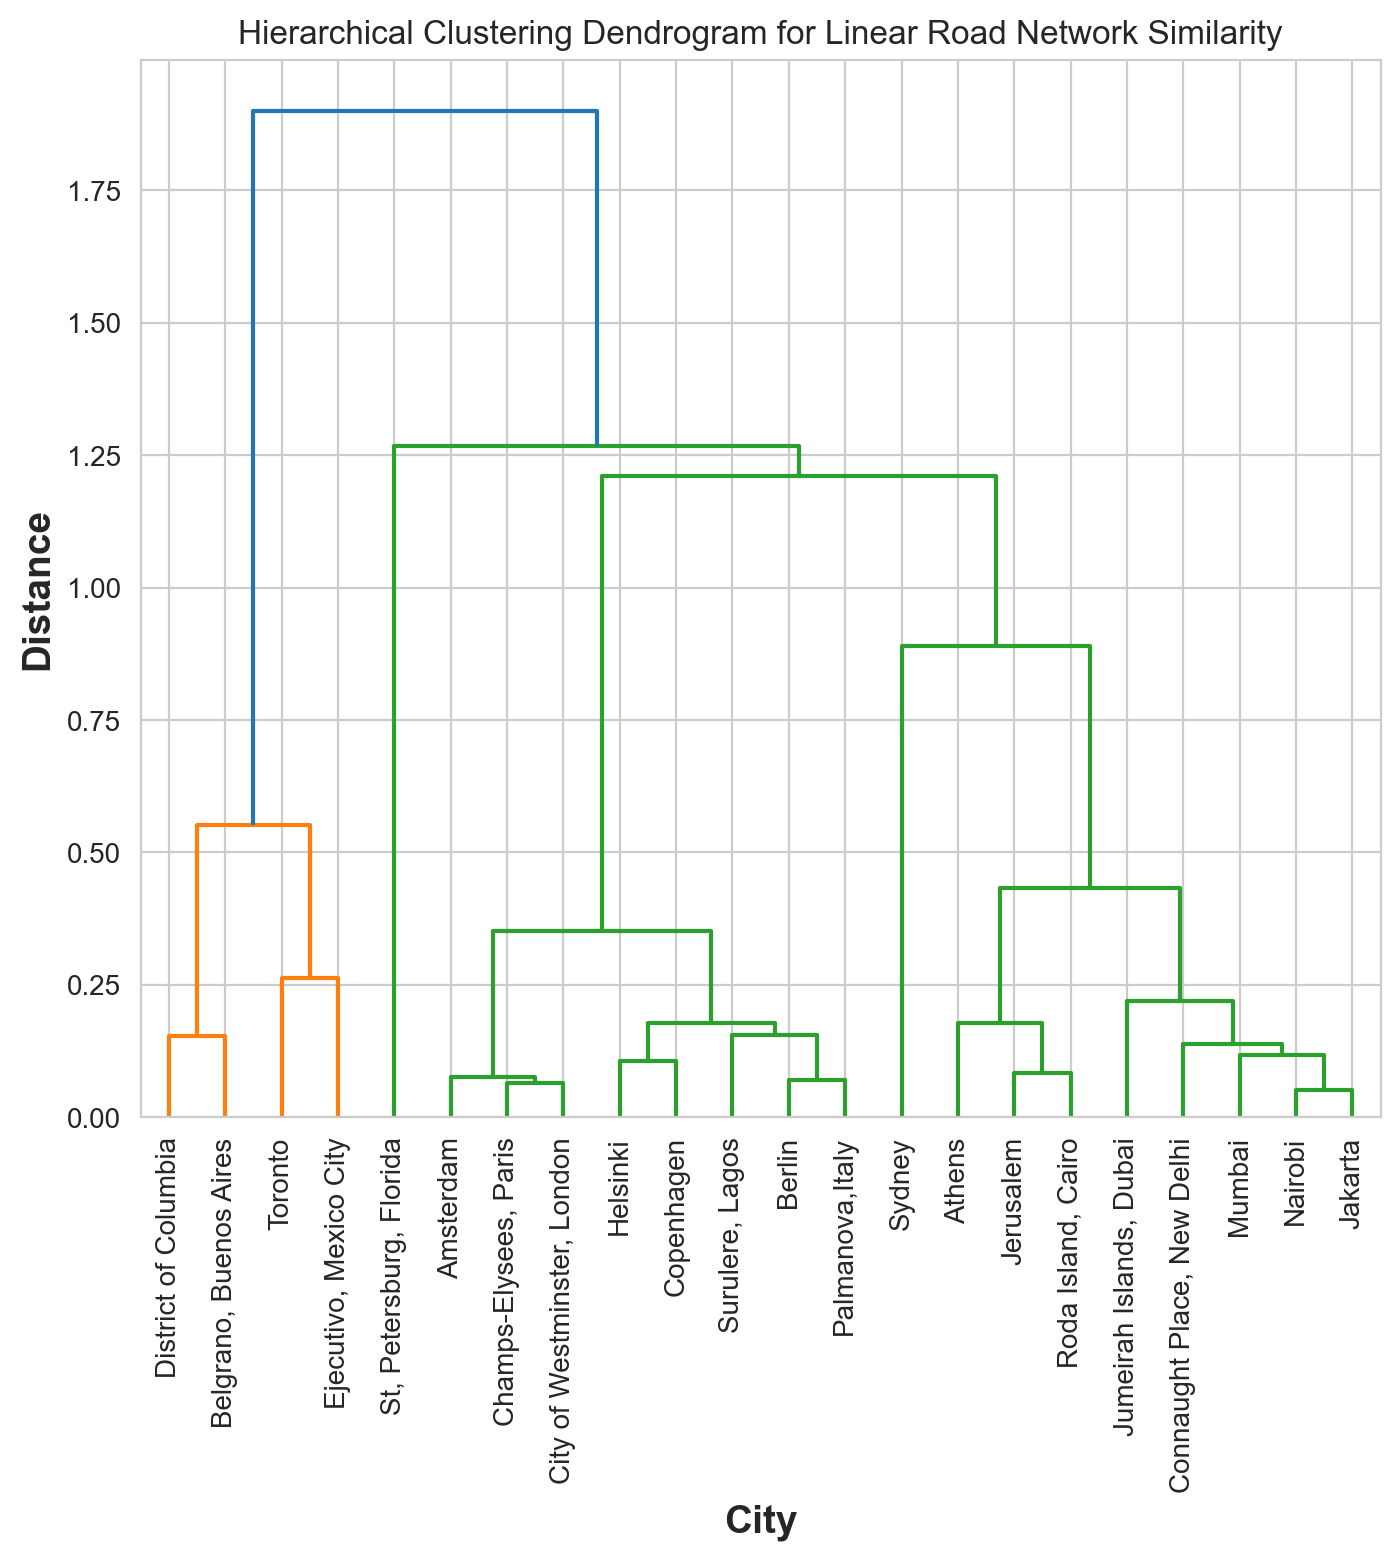
\includegraphics[width=0.75\textwidth,center]{picture/Linear/linear_dendrogram2.png}
\caption[Hierarchical Clustering Dendrogram for Linear Road Networking Similarity]{Hierarchical Clustering Dendrogram for Linear Road Networking Similarity}
\label{fig:Hierarchical Clustering Dendrogram for Linear Road Networking Similarity}
\end{figure}

The dendrogram obtained from the cluster analysis is shown in figure \ref{fig:Hierarchical Clustering Dendrogram for Linear Road Networking Similarity}. The two criteria described in Section 4.1 are used to interpret the dendrogram.

The dendrogram structure reveals two major clusters for the first criteria (Green and Orange). The first criteria, however, fails to interpret the generated clusters because the dendrogram results are not intuitive since some clusters contained a mix of road networks with varying structures. Except for St. Petersburg, Florida, all Road network structures identified through Grid network analysis that have the most pronounced grid-like structure are grouped together (Orange Cluster). Using the second criteria, the road networks of Jakarta and Nairobi are said to be clustered first based on their distances, followed by the cities Champs-Elysees, Paris, City of Westminster, London, and Amsterdam, Netherlands, which are said to be in the same cluster based on their distance, as shown in figure \ref{fig:Hierarchical Clustering Dendrogram for Grid Road Networking Similarity}, \ref{fig:Hierarchical Clustering Dendrogram for Radial Road Networking Similarity} and \ref{fig:Hierarchical Clustering Dendrogram for Tree Road Networking Similarity} respectively which demonstrates a pattern in the similarity methods identifying the similarity between this networks even when the reference networks they are compared to are changed.

In comparison to other Network Structure Analysis, the road networks: Jakarta, Jumeirah Islands, and Dubai, which are identified as the other only linear road network patterns in table \ref{tab:Selected Cities}, are located within the same cluster (green), but further away from the reference road network. This is to be expected because, at a later stage, it is possible to identify the characteristics of the respective cluster and why they were grouped by cross-checking with the similarity scores for each method included in the heatmap in figure \ref{fig:Heatmap showing the correlations for Linear Road Networks}.

\begin{figure}[!ht]
\centering
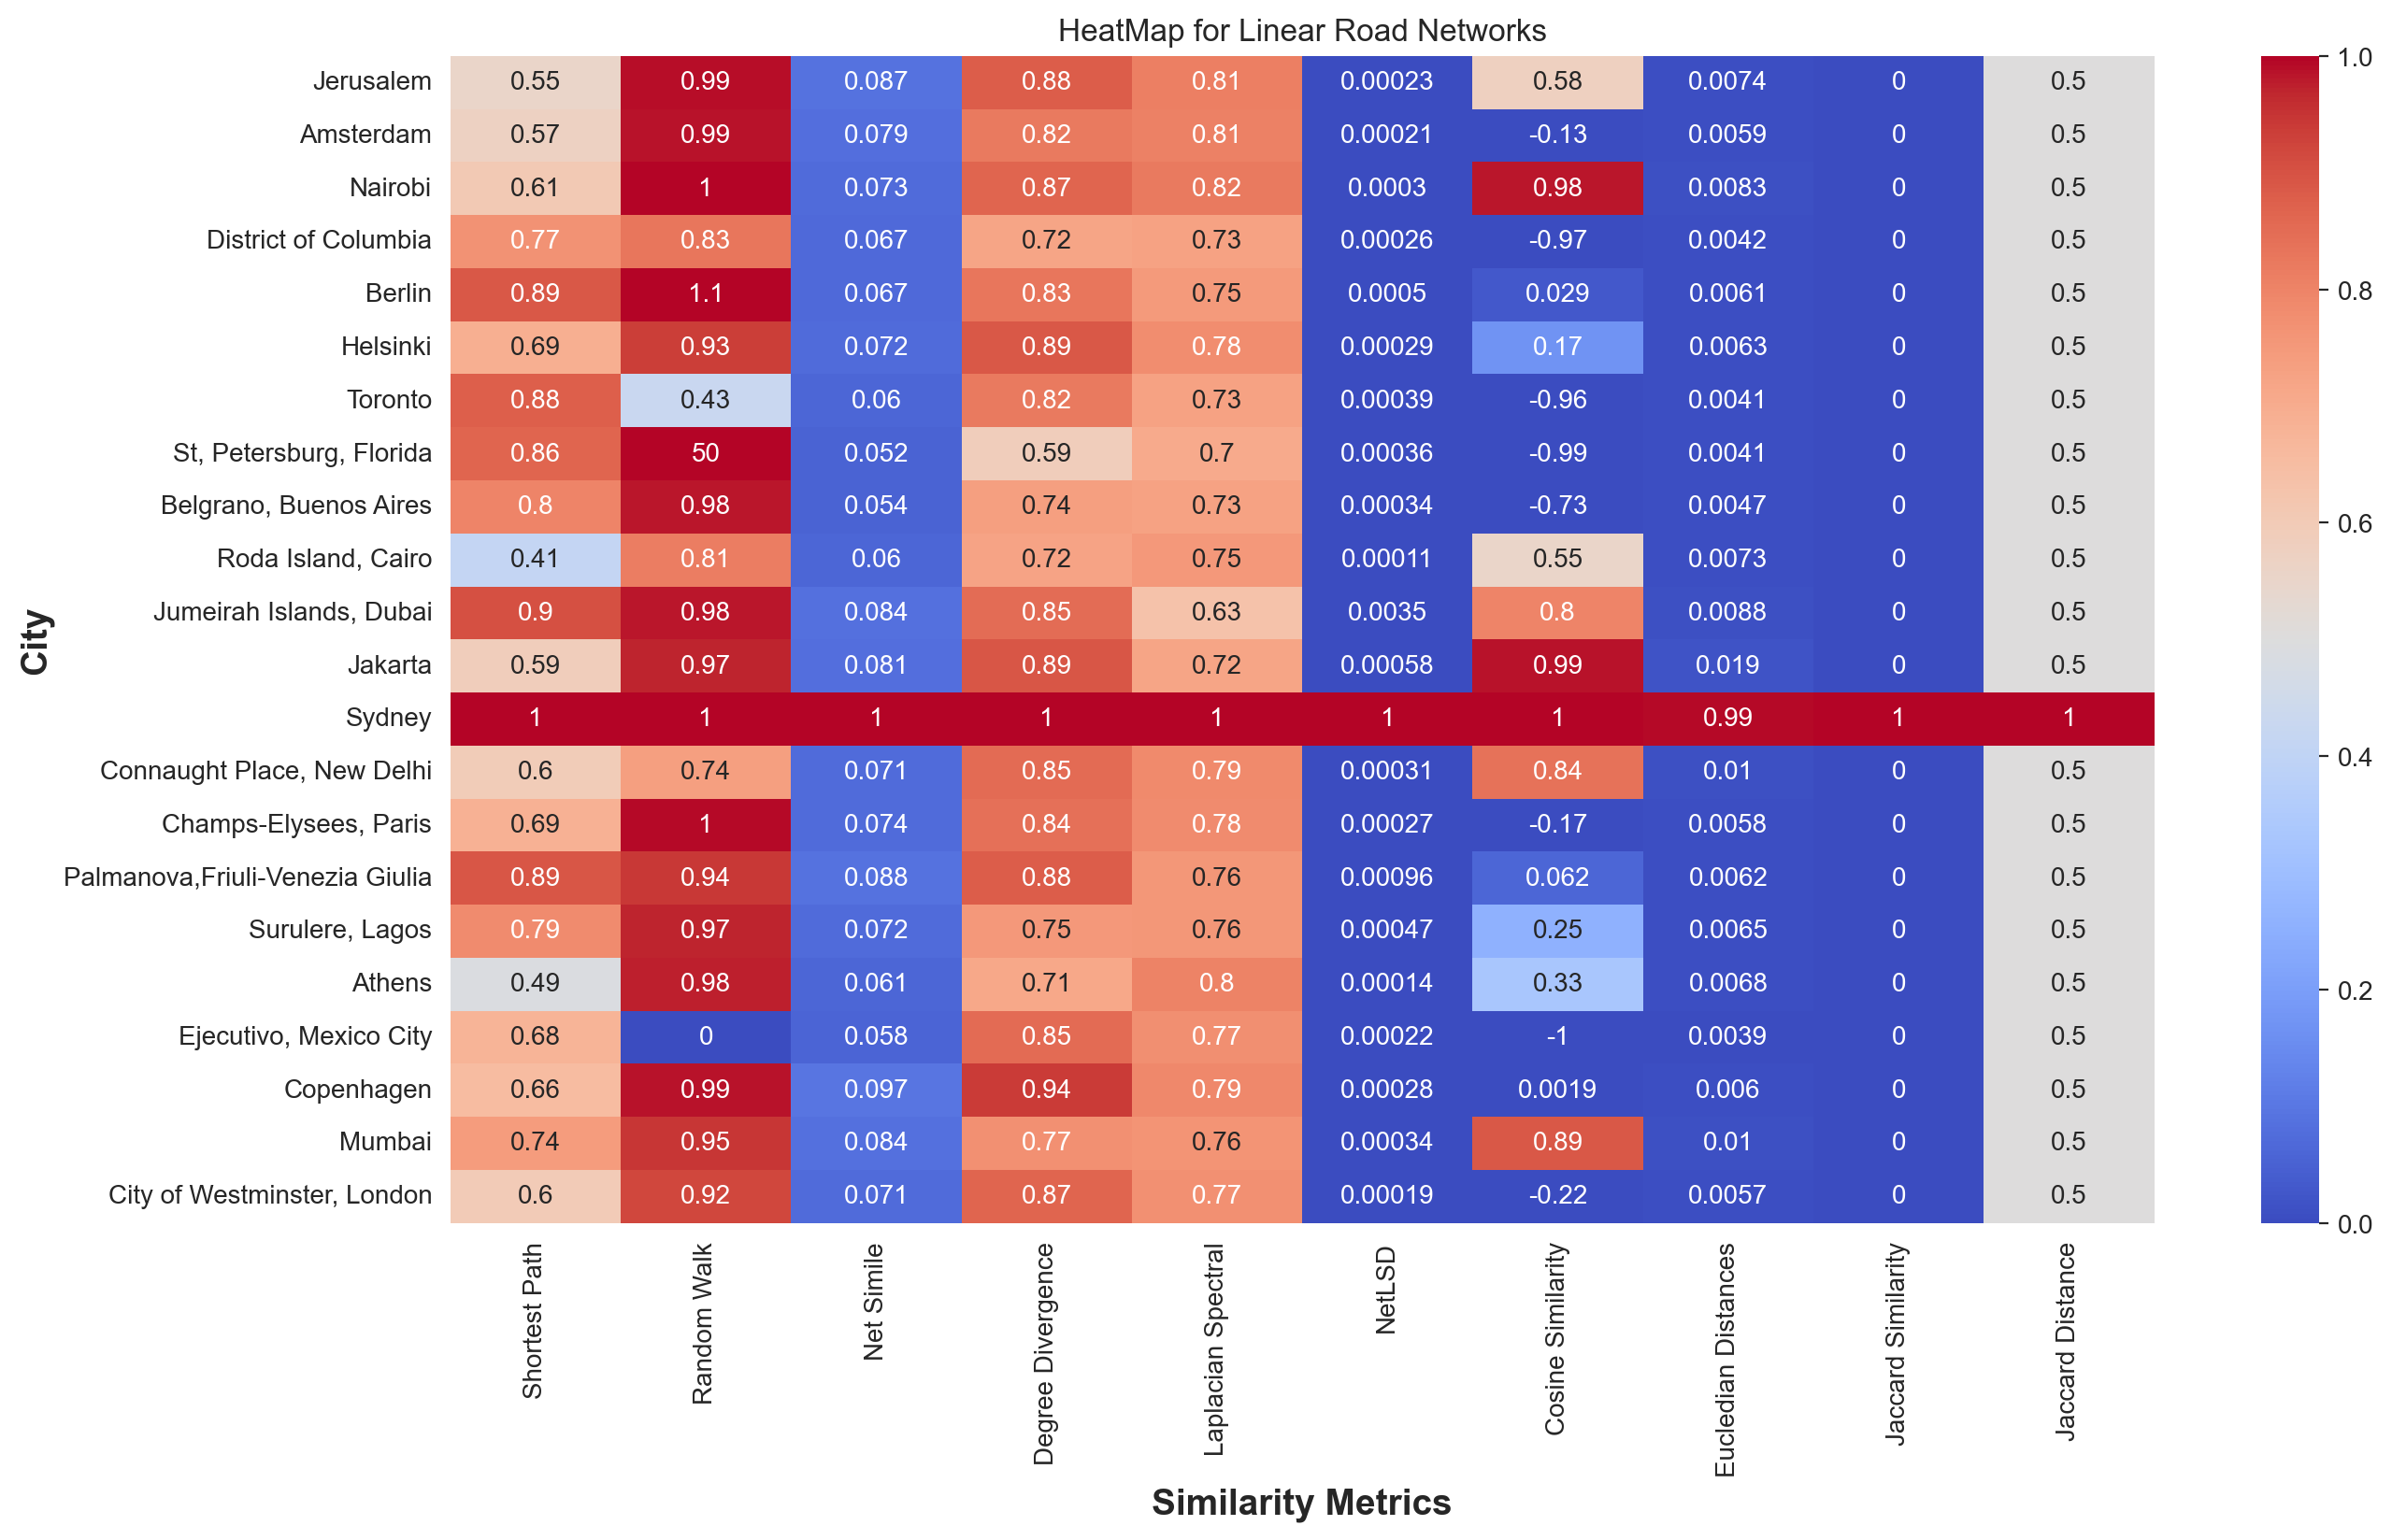
\includegraphics[width=0.85\textwidth,center]{picture/Linear/linearheatmap.png}
\caption[Heatmap showing the correlations for Linear Road Networks]{Heatmap showing the correlations between the road networks when the road network: Sydney (Australia) was used as the reference network.}
\label{fig:Heatmap showing the correlations for Linear Road Networks}
\end{figure}

The pairwise Kendall-Tau distance between each pair of methods is calculated first, followed by a complete-linkage hierarchical clustering because it produces a dendrogram with many small clusters, which provides insight into which groups of methods are closely correlated.

\begin{figure}[!ht]
\centering
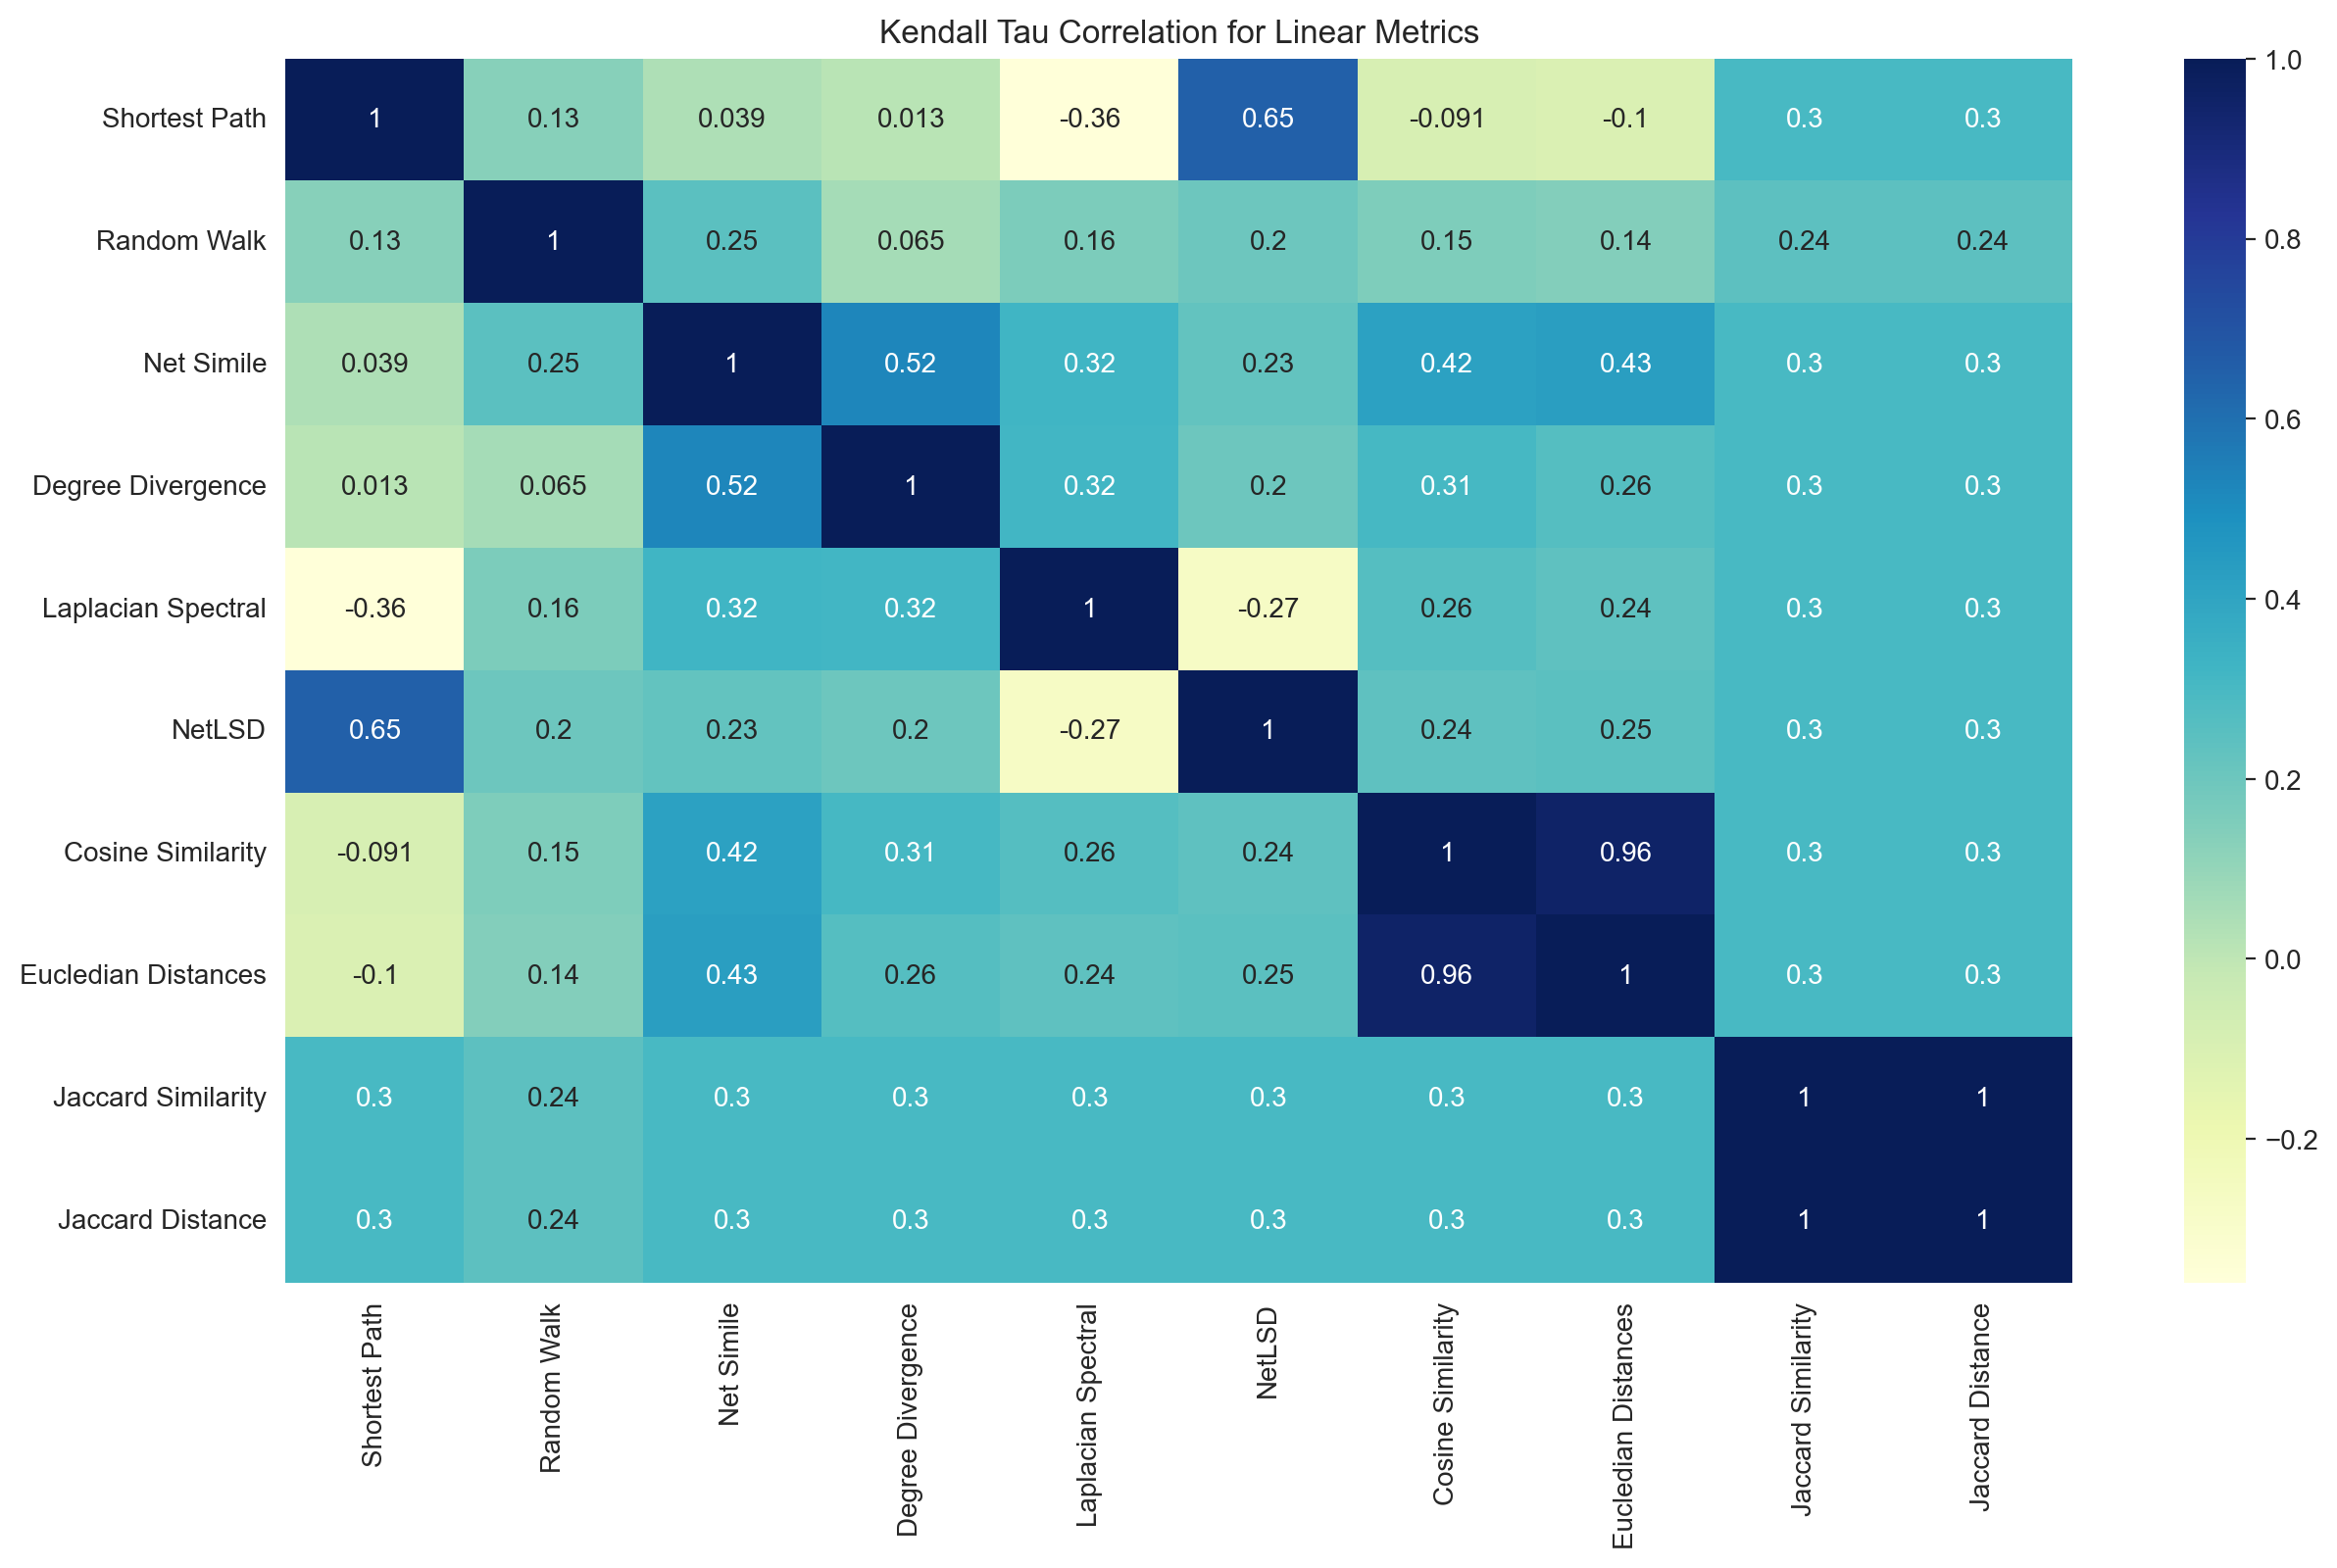
\includegraphics[width=0.85\textwidth,center]{picture/Linear/linear2.png}
\caption[Heatmap showing Kendall-Tau correlations between the road network similarity methods for Linear Road Networks]{Heatmap showing Kendall-Tau correlations between the road network similarity methods when the road network: Sydney (Australia) was used as the reference network.}
\label{fig:network ranking linear}
\end{figure}

The results for the Kendall Tau distances between the scores are very similar to the previous analysis, albeit with slightly different numbers.

Figure \ref{fig:network ranking linear} depicts the Kendall-Tau distances between the scores generated by the various methods when comparing road networks similar to the reference network with a Linear like structure. When both the Jaccard Distance and the Jaccard Similarity are used, the results show a one-to-one positive correlation. Again, this is understandable given that the Jaccard Distance is thought to be complementary to the Jaccard Similarity, which is calculated by subtracting the Jaccard coefficient from 1. The methods cosine similarity and euclidean distance also behave similarly, with a correlation of 0.96. Both methods are vector-based and operate at the micro level, as shown in table \ref{tab:Road Network Similarity Methods}. This means that either of the two methods could be used to calculate vector-based similarity on road networks at the Micro-level. The other methods, on the other hand, have a much weaker correlation because the level of the network they operate on and the type of comparison they use are different.

\section{Cul de Sac Road Network Similarity Analysis}

For the Cul de Sac road similarity analysis, the road network Jerusalem (Israel) was chosen as the reference network, and the methods are used to compare the other networks to the reference network and generate a numerical similarity score. The networks are then organized into hierarchical clusters. Figure \ref{fig:Hierarchical Clustering Dendrogram for Cul De Sac Road Networking Similarity} shows the results of this analysis.

\begin{figure}[!ht]
\centering
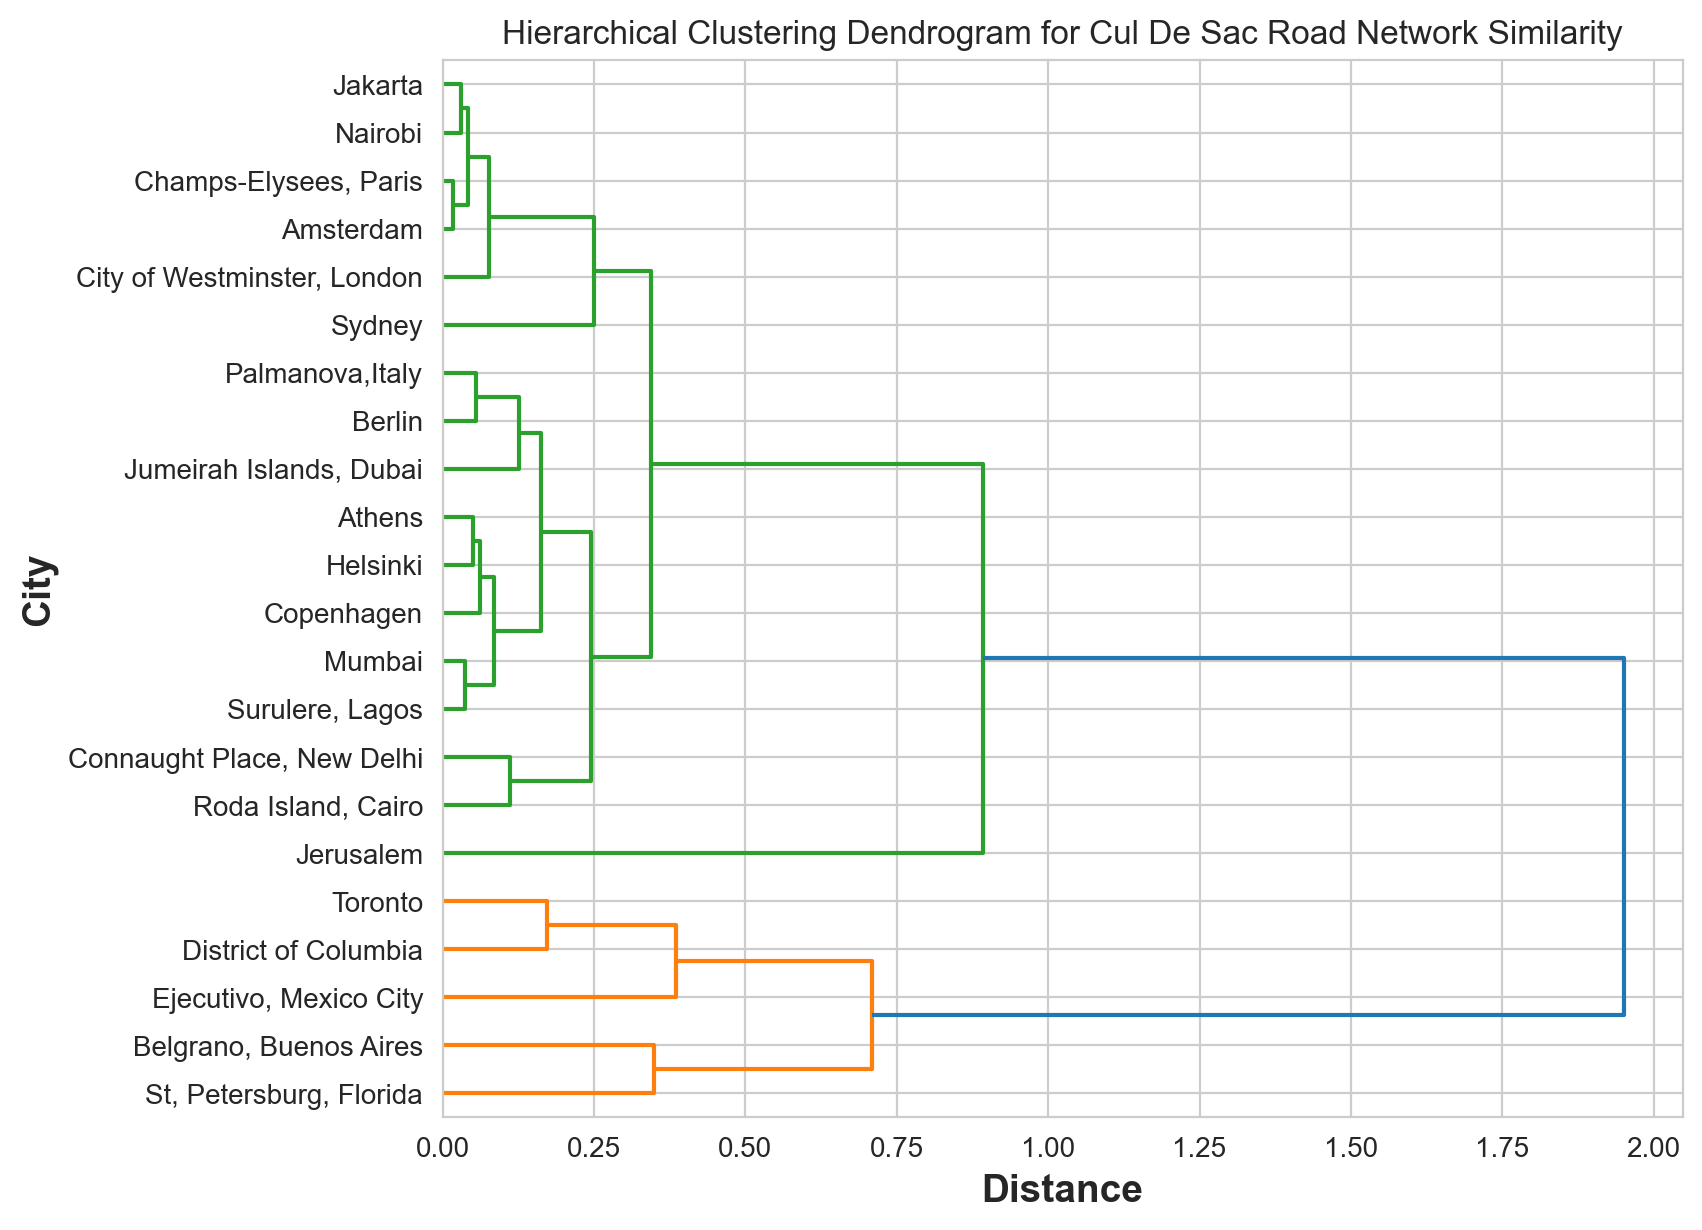
\includegraphics[width=0.75\textwidth,center]{picture/Cul De Sac/culdesac_dendrogram2.png}
\caption[Hierarchical Clustering Dendrogram for Cul De Sac Road Networking Similarity]{Hierarchical Clustering Dendrogram for Cul De Sac Road Networking Similarity}
\label{fig:Hierarchical Clustering Dendrogram for Cul De Sac Road Networking Similarity}
\end{figure}

The dendrogram obtained from the cluster analysis is shown in figure \ref{fig:Hierarchical Clustering Dendrogram for Cul De Sac Road Networking Similarity}. The two criteria described in Section 4.1 are used to interpret the dendrogram.

The dendrogram structure reveals two major clusters for the first criterion (Green and Orange). The first criteria, however, fails to interpret the generated clusters because the dendrogram results are not intuitive since some clusters contained a mix of road networks with varying structures. However, all Road network structures identified by Grid network analysis that have the most pronounced grid-like structure are grouped together (Orange Cluster). Interpreting the dendrogram using the second criteria, the road networks for the cities Champs-Elysees, Paris, City of Westminster, and Amsterdam, Netherland are said to be clustered first based on their distances, which are similar to figures \ref{fig:Hierarchical Clustering Dendrogram for Grid Road Networking Similarity}, \ref{fig:Hierarchical Clustering Dendrogram for Radial Road Networking Similarity}, \ref{fig:Hierarchical Clustering Dendrogram for Tree Road Networking Similarity}, \ref{fig:Hierarchical Clustering Dendrogram for Linear Road Networking Similarity} and  followed by the cities Jakarta and Nairobi are said to be in the same cluster based on their distances  respectively which demonstrates a pattern in the similarity methods identifying the similarity between this networks even when the reference networks they are compared to are changed.

In comparison to the other Network Analysis, the road network: Amsterdam, which is identified as the other only cul de sac road network pattern in table  \ref{tab:Selected Cities}, is located within the same cluster (green), but further away from the reference road network. This is to be expected because it is possible to identify the characteristics of each cluster and why they are not grouped together by cross-checking the similarity scores for each method included in the heatmap in rfigure \ref{fig:Heatmap showing the correlations for Tree Road Networks}.


\begin{figure}[!ht]
\centering
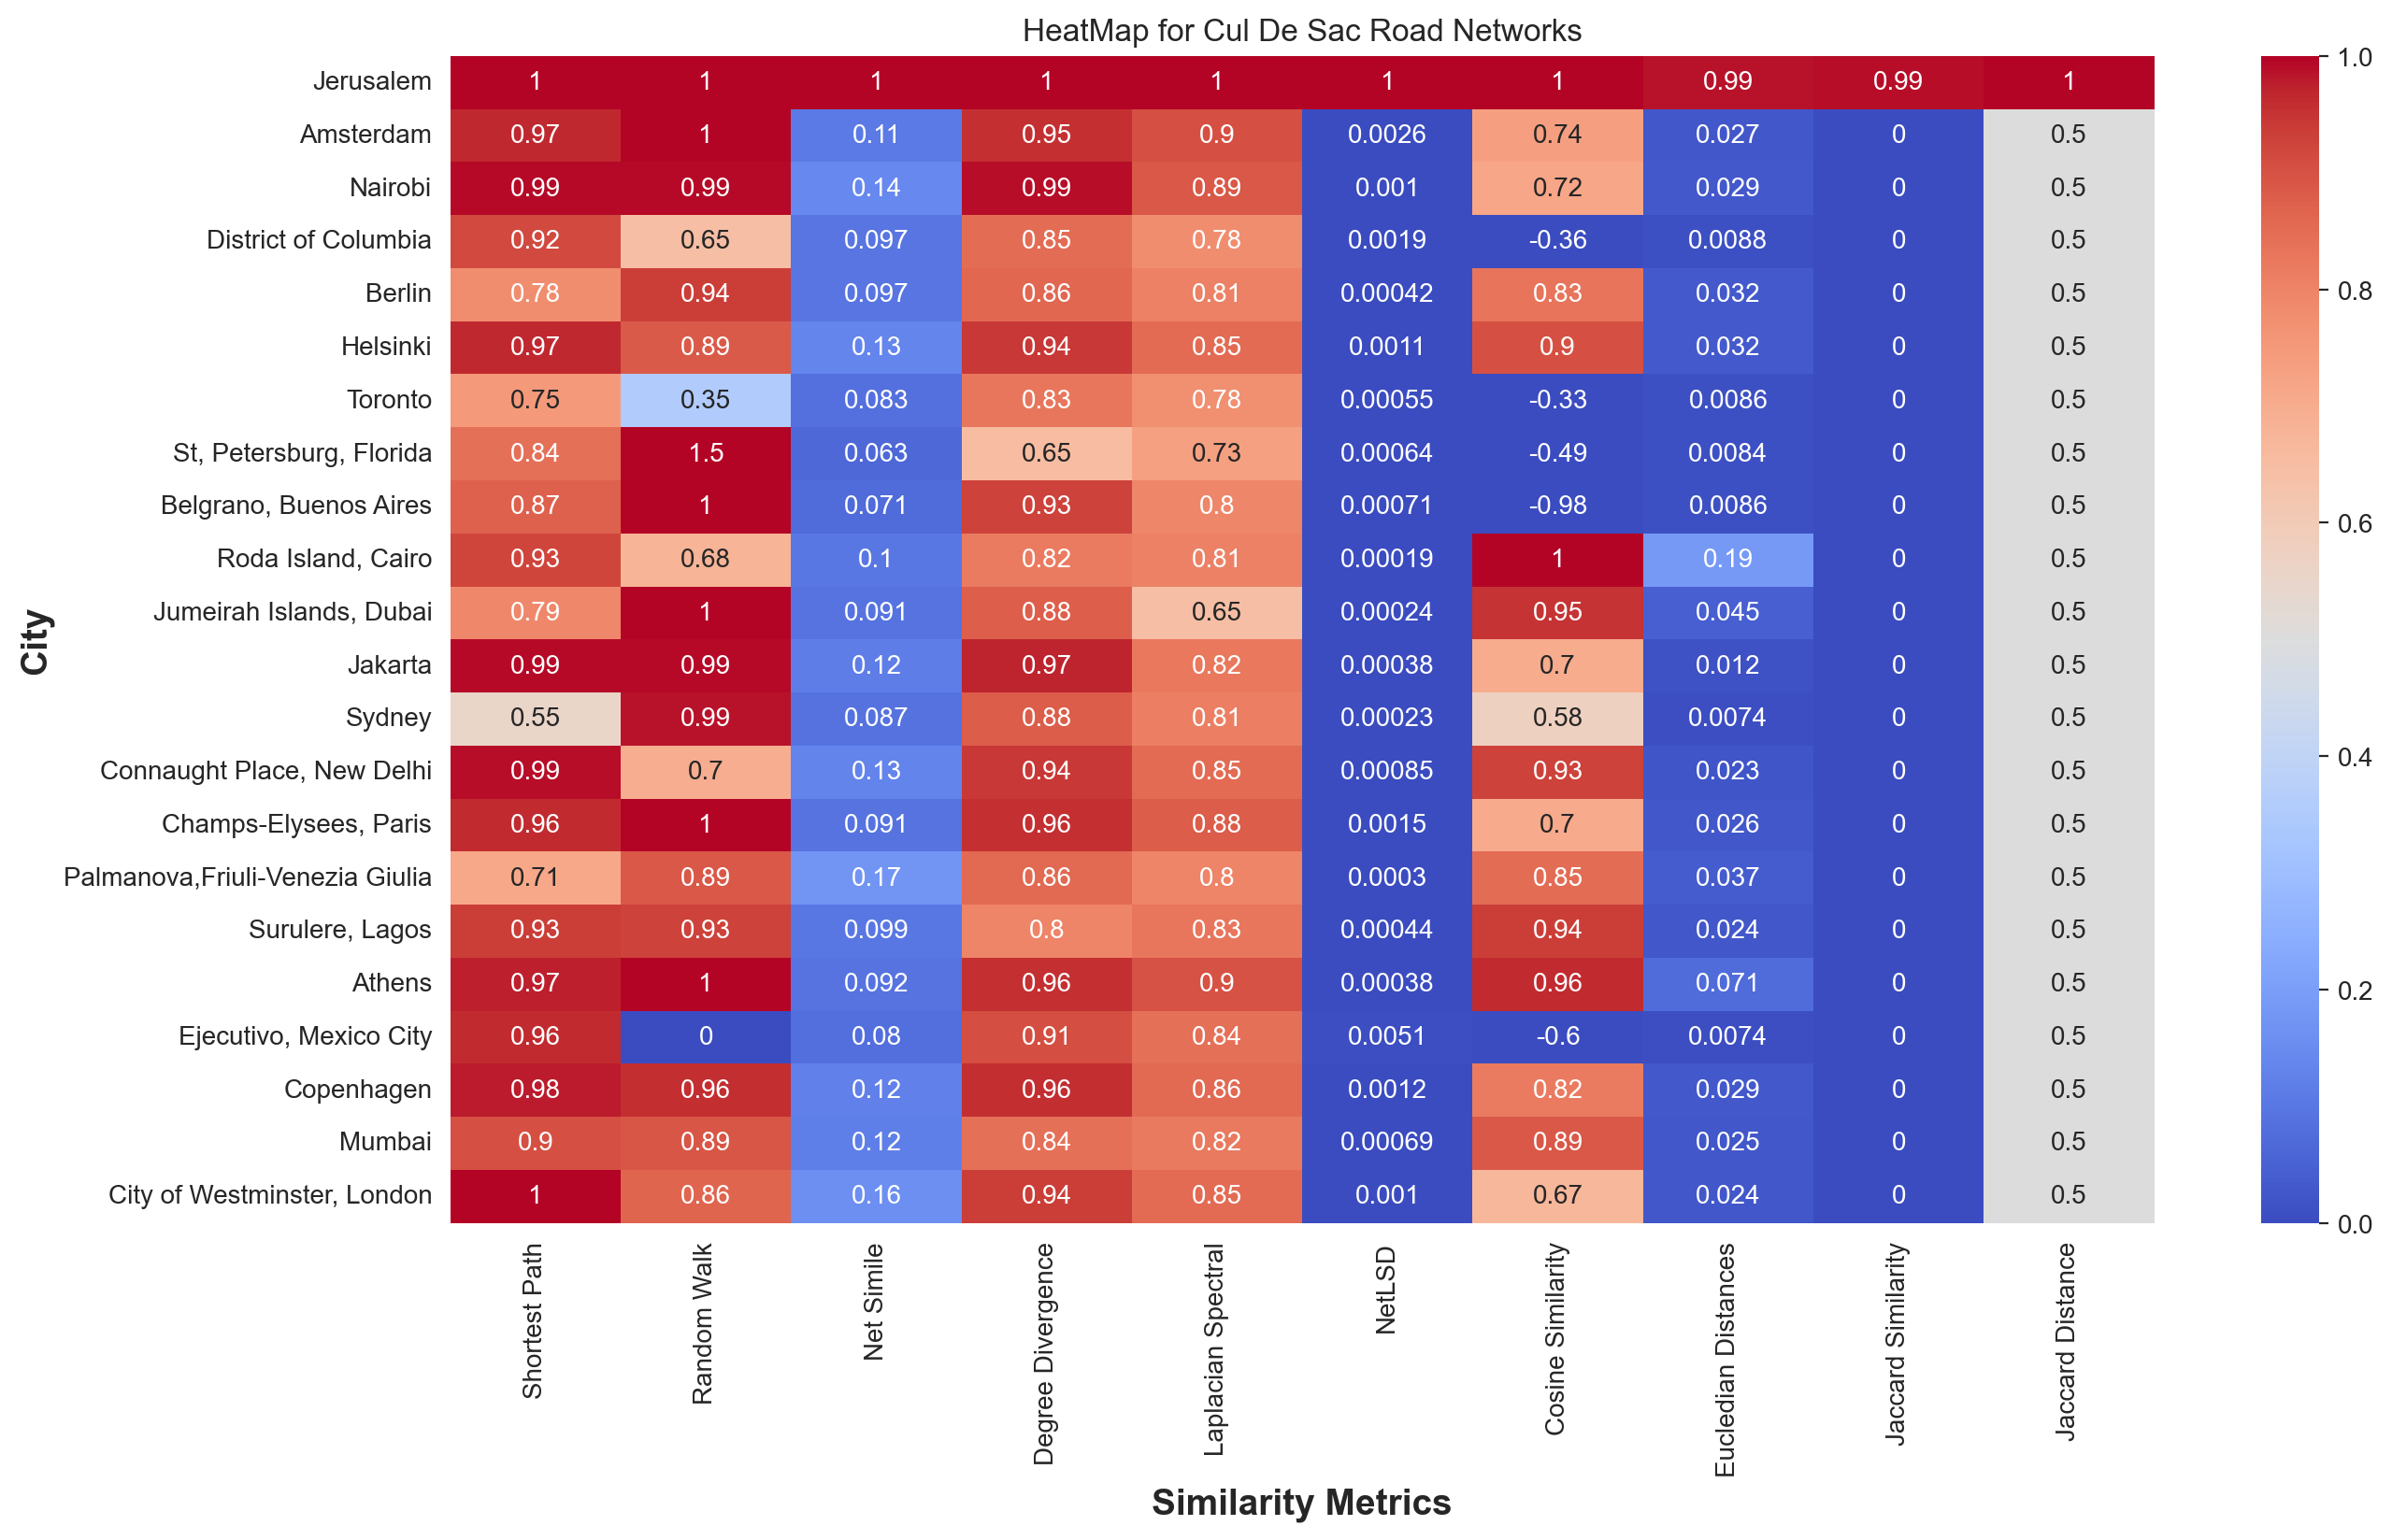
\includegraphics[width=0.85\textwidth,center]{picture/Cul De Sac/culdesacheatmap.png}
\caption[Heatmap showing the correlations for Cul De Sac Road Networks]{Heatmap showing the correlations between the road networks when the road network: Jerusalem (Israel) was used as the reference network.}
\label{fig:Heatmap showing the correlations for Cul De Sac Road Networks}
\end{figure}

The pairwise Kendall-Tau distance between each pair of methods is calculated first, followed by a complete-linkage hierarchical clustering because it produces a dendrogram with many small clusters, which provides insight into which groups of methods are closely correlated.

\begin{figure}[!ht]
\centering
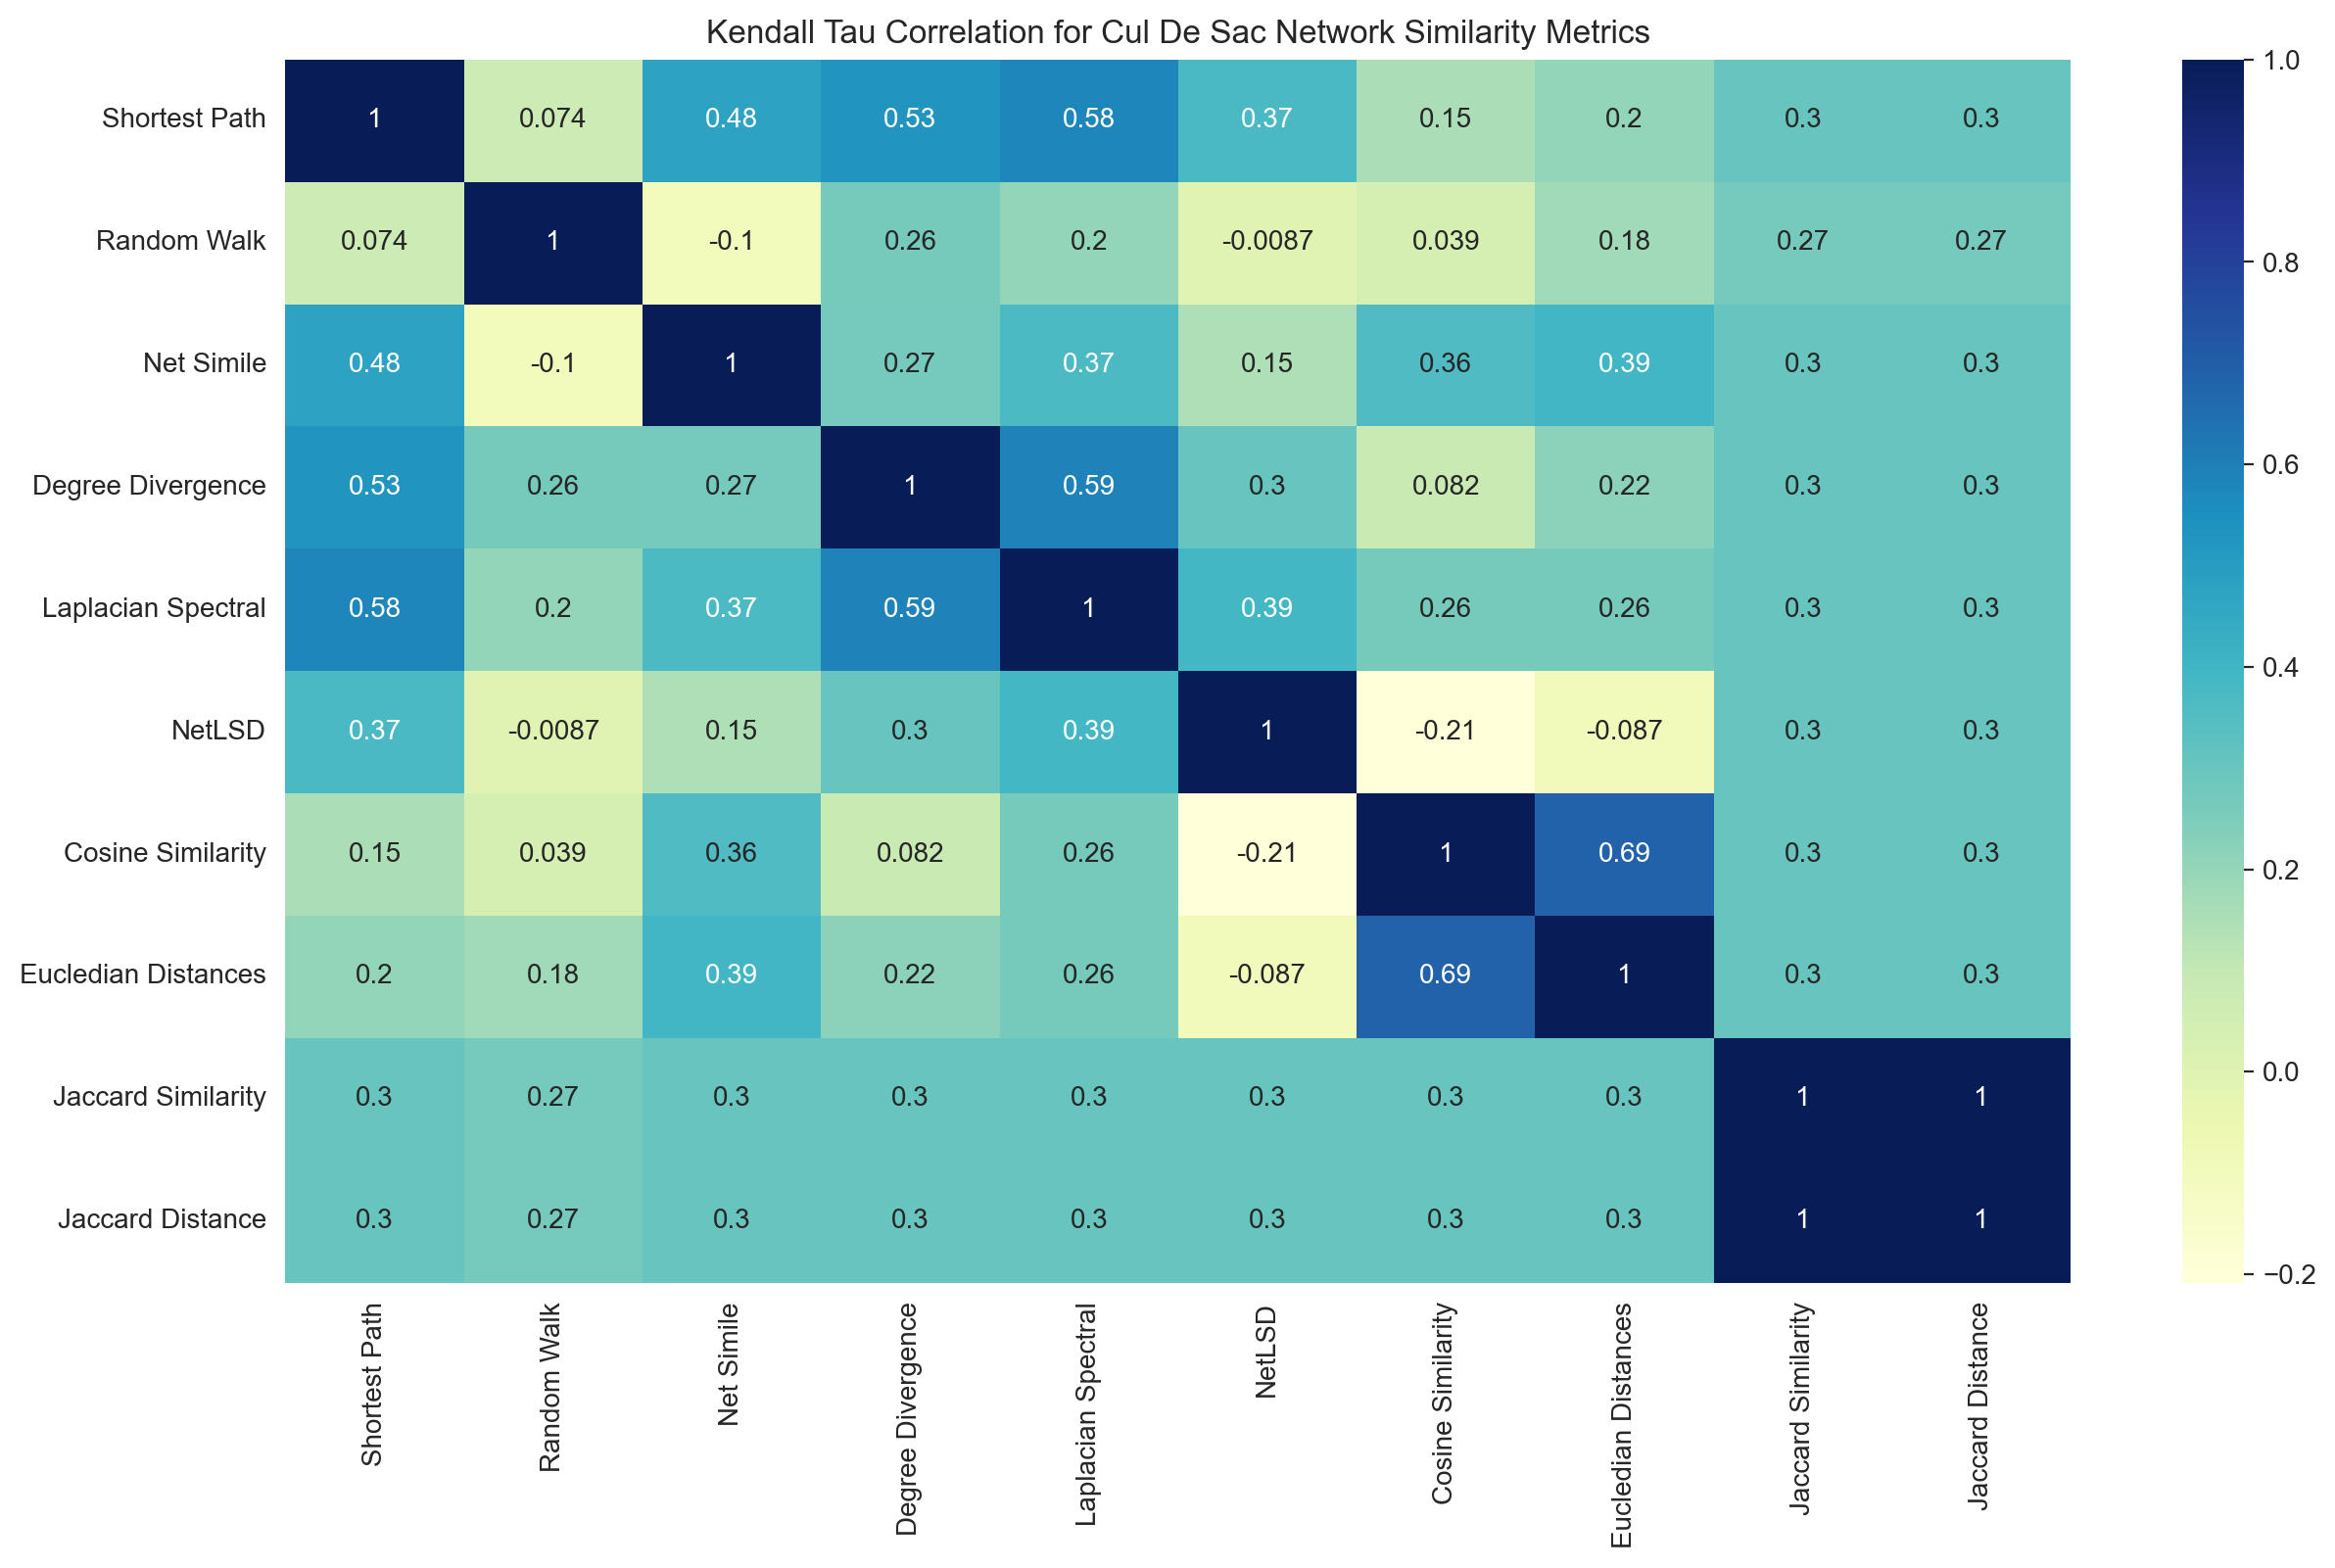
\includegraphics[width=0.85\textwidth,center]{picture/Cul De Sac/culdesac2.png}
\caption[Heatmap showing Kendall-Tau correlations between the road network similarity methods for Cul De Sac Road Networks]{Heatmap showing Kendall-Tau correlations between the road network similarity methods when the road network: Jerusalem, Israel was used as the reference network.}
\label{fig:network ranking Cul De Sac}
\end{figure}

The results for the Kendall Tau distances between the scores are very similar to the previous analysis, albeit with slightly different numbers. Figure \ref{fig:network ranking linear} depicts the Kendall-Tau distances between the scores generated by the various methods when comparing road networks similar to the reference network with a Tree-like structure. When both the Jaccard Distance and the Jaccard Similarity are used, the results show a one-to-one positive correlation. This is understandable given that the Jaccard Distance is thought to be complementary to the Jaccard Similarity, which is calculated by subtracting the Jaccard coefficient from 1. The methods cosine similarity and euclidean distance behave differently than other results, with a correlation of 0.69. The reason for this change could not be determined in this study, but it could be considered in future research. The other methods, however, have a significantly weaker correlation because the level of the network they all operate on and the type of comparison they use differ.